\documentclass[]{book}
\usepackage{lmodern}
\usepackage{amssymb,amsmath}
\usepackage{ifxetex,ifluatex}
\usepackage{fixltx2e} % provides \textsubscript
\ifnum 0\ifxetex 1\fi\ifluatex 1\fi=0 % if pdftex
  \usepackage[T1]{fontenc}
  \usepackage[utf8]{inputenc}
\else % if luatex or xelatex
  \ifxetex
    \usepackage{mathspec}
  \else
    \usepackage{fontspec}
  \fi
  \defaultfontfeatures{Ligatures=TeX,Scale=MatchLowercase}
\fi
% use upquote if available, for straight quotes in verbatim environments
\IfFileExists{upquote.sty}{\usepackage{upquote}}{}
% use microtype if available
\IfFileExists{microtype.sty}{%
\usepackage{microtype}
\UseMicrotypeSet[protrusion]{basicmath} % disable protrusion for tt fonts
}{}
\usepackage[margin=1in]{geometry}
\usepackage{hyperref}
\hypersetup{unicode=true,
            pdftitle={R notes},
            pdfauthor={Lucy Liu},
            pdfborder={0 0 0},
            breaklinks=true}
\urlstyle{same}  % don't use monospace font for urls
\usepackage{natbib}
\bibliographystyle{plainnat}
\usepackage{color}
\usepackage{fancyvrb}
\newcommand{\VerbBar}{|}
\newcommand{\VERB}{\Verb[commandchars=\\\{\}]}
\DefineVerbatimEnvironment{Highlighting}{Verbatim}{commandchars=\\\{\}}
% Add ',fontsize=\small' for more characters per line
\usepackage{framed}
\definecolor{shadecolor}{RGB}{248,248,248}
\newenvironment{Shaded}{\begin{snugshade}}{\end{snugshade}}
\newcommand{\KeywordTok}[1]{\textcolor[rgb]{0.13,0.29,0.53}{\textbf{#1}}}
\newcommand{\DataTypeTok}[1]{\textcolor[rgb]{0.13,0.29,0.53}{#1}}
\newcommand{\DecValTok}[1]{\textcolor[rgb]{0.00,0.00,0.81}{#1}}
\newcommand{\BaseNTok}[1]{\textcolor[rgb]{0.00,0.00,0.81}{#1}}
\newcommand{\FloatTok}[1]{\textcolor[rgb]{0.00,0.00,0.81}{#1}}
\newcommand{\ConstantTok}[1]{\textcolor[rgb]{0.00,0.00,0.00}{#1}}
\newcommand{\CharTok}[1]{\textcolor[rgb]{0.31,0.60,0.02}{#1}}
\newcommand{\SpecialCharTok}[1]{\textcolor[rgb]{0.00,0.00,0.00}{#1}}
\newcommand{\StringTok}[1]{\textcolor[rgb]{0.31,0.60,0.02}{#1}}
\newcommand{\VerbatimStringTok}[1]{\textcolor[rgb]{0.31,0.60,0.02}{#1}}
\newcommand{\SpecialStringTok}[1]{\textcolor[rgb]{0.31,0.60,0.02}{#1}}
\newcommand{\ImportTok}[1]{#1}
\newcommand{\CommentTok}[1]{\textcolor[rgb]{0.56,0.35,0.01}{\textit{#1}}}
\newcommand{\DocumentationTok}[1]{\textcolor[rgb]{0.56,0.35,0.01}{\textbf{\textit{#1}}}}
\newcommand{\AnnotationTok}[1]{\textcolor[rgb]{0.56,0.35,0.01}{\textbf{\textit{#1}}}}
\newcommand{\CommentVarTok}[1]{\textcolor[rgb]{0.56,0.35,0.01}{\textbf{\textit{#1}}}}
\newcommand{\OtherTok}[1]{\textcolor[rgb]{0.56,0.35,0.01}{#1}}
\newcommand{\FunctionTok}[1]{\textcolor[rgb]{0.00,0.00,0.00}{#1}}
\newcommand{\VariableTok}[1]{\textcolor[rgb]{0.00,0.00,0.00}{#1}}
\newcommand{\ControlFlowTok}[1]{\textcolor[rgb]{0.13,0.29,0.53}{\textbf{#1}}}
\newcommand{\OperatorTok}[1]{\textcolor[rgb]{0.81,0.36,0.00}{\textbf{#1}}}
\newcommand{\BuiltInTok}[1]{#1}
\newcommand{\ExtensionTok}[1]{#1}
\newcommand{\PreprocessorTok}[1]{\textcolor[rgb]{0.56,0.35,0.01}{\textit{#1}}}
\newcommand{\AttributeTok}[1]{\textcolor[rgb]{0.77,0.63,0.00}{#1}}
\newcommand{\RegionMarkerTok}[1]{#1}
\newcommand{\InformationTok}[1]{\textcolor[rgb]{0.56,0.35,0.01}{\textbf{\textit{#1}}}}
\newcommand{\WarningTok}[1]{\textcolor[rgb]{0.56,0.35,0.01}{\textbf{\textit{#1}}}}
\newcommand{\AlertTok}[1]{\textcolor[rgb]{0.94,0.16,0.16}{#1}}
\newcommand{\ErrorTok}[1]{\textcolor[rgb]{0.64,0.00,0.00}{\textbf{#1}}}
\newcommand{\NormalTok}[1]{#1}
\usepackage{longtable,booktabs}
\usepackage{graphicx,grffile}
\makeatletter
\def\maxwidth{\ifdim\Gin@nat@width>\linewidth\linewidth\else\Gin@nat@width\fi}
\def\maxheight{\ifdim\Gin@nat@height>\textheight\textheight\else\Gin@nat@height\fi}
\makeatother
% Scale images if necessary, so that they will not overflow the page
% margins by default, and it is still possible to overwrite the defaults
% using explicit options in \includegraphics[width, height, ...]{}
\setkeys{Gin}{width=\maxwidth,height=\maxheight,keepaspectratio}
\IfFileExists{parskip.sty}{%
\usepackage{parskip}
}{% else
\setlength{\parindent}{0pt}
\setlength{\parskip}{6pt plus 2pt minus 1pt}
}
\setlength{\emergencystretch}{3em}  % prevent overfull lines
\providecommand{\tightlist}{%
  \setlength{\itemsep}{0pt}\setlength{\parskip}{0pt}}
\setcounter{secnumdepth}{5}
% Redefines (sub)paragraphs to behave more like sections
\ifx\paragraph\undefined\else
\let\oldparagraph\paragraph
\renewcommand{\paragraph}[1]{\oldparagraph{#1}\mbox{}}
\fi
\ifx\subparagraph\undefined\else
\let\oldsubparagraph\subparagraph
\renewcommand{\subparagraph}[1]{\oldsubparagraph{#1}\mbox{}}
\fi

%%% Use protect on footnotes to avoid problems with footnotes in titles
\let\rmarkdownfootnote\footnote%
\def\footnote{\protect\rmarkdownfootnote}

%%% Change title format to be more compact
\usepackage{titling}

% Create subtitle command for use in maketitle
\newcommand{\subtitle}[1]{
  \posttitle{
    \begin{center}\large#1\end{center}
    }
}

\setlength{\droptitle}{-2em}

  \title{R notes}
    \pretitle{\vspace{\droptitle}\centering\huge}
  \posttitle{\par}
    \author{Lucy Liu}
    \preauthor{\centering\large\emph}
  \postauthor{\par}
      \predate{\centering\large\emph}
  \postdate{\par}
    \date{2018-12-19}

\usepackage{booktabs}
\usepackage{amsthm}
\makeatletter
\def\thm@space@setup{%
  \thm@preskip=8pt plus 2pt minus 4pt
  \thm@postskip=\thm@preskip
}
\makeatother

\begin{document}
\maketitle

{
\setcounter{tocdepth}{1}
\tableofcontents
}
These are my notes on R.

\chapter{Base R}\label{base-r}

\chapter{ggplot2}\label{ggplot2}

Useful references:

\begin{itemize}
\tightlist
\item
  \href{https://www.ggplot2-exts.org}{ggplot2 extensions}
\item
  \href{http://ggplot2.tidyverse.org/reference/}{Theory of ggplot}
\item
  \href{https://rstudio-pubs-static.s3.amazonaws.com/3364_d1a578f521174152b46b19d0c83cbe7e.html}{Themes}
\end{itemize}

\section{Introduction}\label{introduction}

The general syntax of a ggplot2 call:

\begin{Shaded}
\begin{Highlighting}[]
\KeywordTok{ggplot}\NormalTok{(}\DataTypeTok{data =} \OperatorTok{<}\NormalTok{DATA}\OperatorTok{>}\NormalTok{) }\OperatorTok{+}\StringTok{ }
\StringTok{  }\ErrorTok{<}\NormalTok{GEOM_FUNCTION}\OperatorTok{>}\NormalTok{(}
     \DataTypeTok{mapping =} \KeywordTok{aes}\NormalTok{(}\OperatorTok{<}\NormalTok{MAPPINGS}\OperatorTok{>}\NormalTok{),}
     \DataTypeTok{stat =} \OperatorTok{<}\NormalTok{STAT}\OperatorTok{>}\NormalTok{,    }\CommentTok{#statistical transformation}
     \DataTypeTok{position =} \OperatorTok{<}\NormalTok{POSITION}\OperatorTok{>}\NormalTok{) }\OperatorTok{+}
\StringTok{  }\ErrorTok{<}\NormalTok{COORDINATE_FUNCTION}\OperatorTok{>}\StringTok{ }\OperatorTok{+}
\StringTok{  }\ErrorTok{<}\NormalTok{FACET_FUNCTION}\OperatorTok{>}
\end{Highlighting}
\end{Shaded}

There are 7 parameters to specify but you will rarely have to specify
all 7 parameters as ggplot has useful defaults.

\subsection{geoms}\label{geoms}

Different types of graphs are called different `geoms', as they can be
thought of geometrical objects used to represent data. E.g.:

\begin{itemize}
\tightlist
\item
  geom\_bar = bar graph
\item
  geom\_line = line graph
\item
  geom\_boxplot = box plot\\
\item
  geom\_point = scatter plot
\item
  geom\_smooth = smooth line fitted to the data
\end{itemize}

\subsection{Layering}\label{layering}

Think of ggplot2 as creating a plot using layers. Here is a simple
scatter plot:

\begin{Shaded}
\begin{Highlighting}[]
\KeywordTok{ggplot}\NormalTok{(}\DataTypeTok{data =}\NormalTok{ mpg) }\OperatorTok{+}\StringTok{ }
\StringTok{  }\KeywordTok{geom_point}\NormalTok{(}\DataTypeTok{mapping =} \KeywordTok{aes}\NormalTok{(}\DataTypeTok{x =}\NormalTok{ displ, }\DataTypeTok{y =}\NormalTok{ hwy))}
\end{Highlighting}
\end{Shaded}

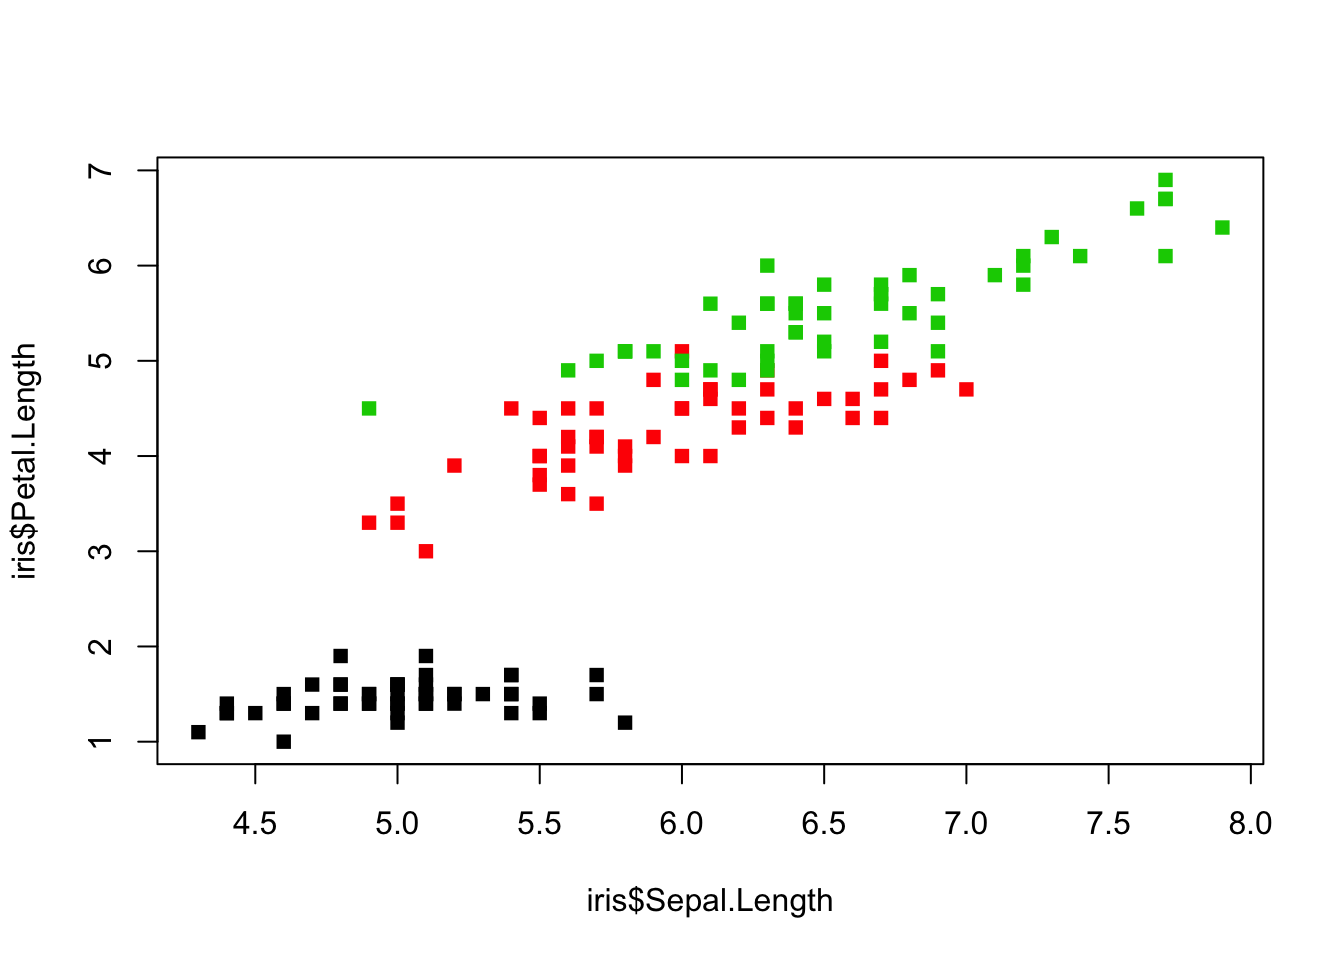
\includegraphics{R_notes_files/figure-latex/unnamed-chunk-3-1.pdf}

We can break this down into `layers'.

This creates an empty graph:

\begin{Shaded}
\begin{Highlighting}[]
\KeywordTok{ggplot}\NormalTok{(}\DataTypeTok{data=}\NormalTok{mpg)}
\end{Highlighting}
\end{Shaded}

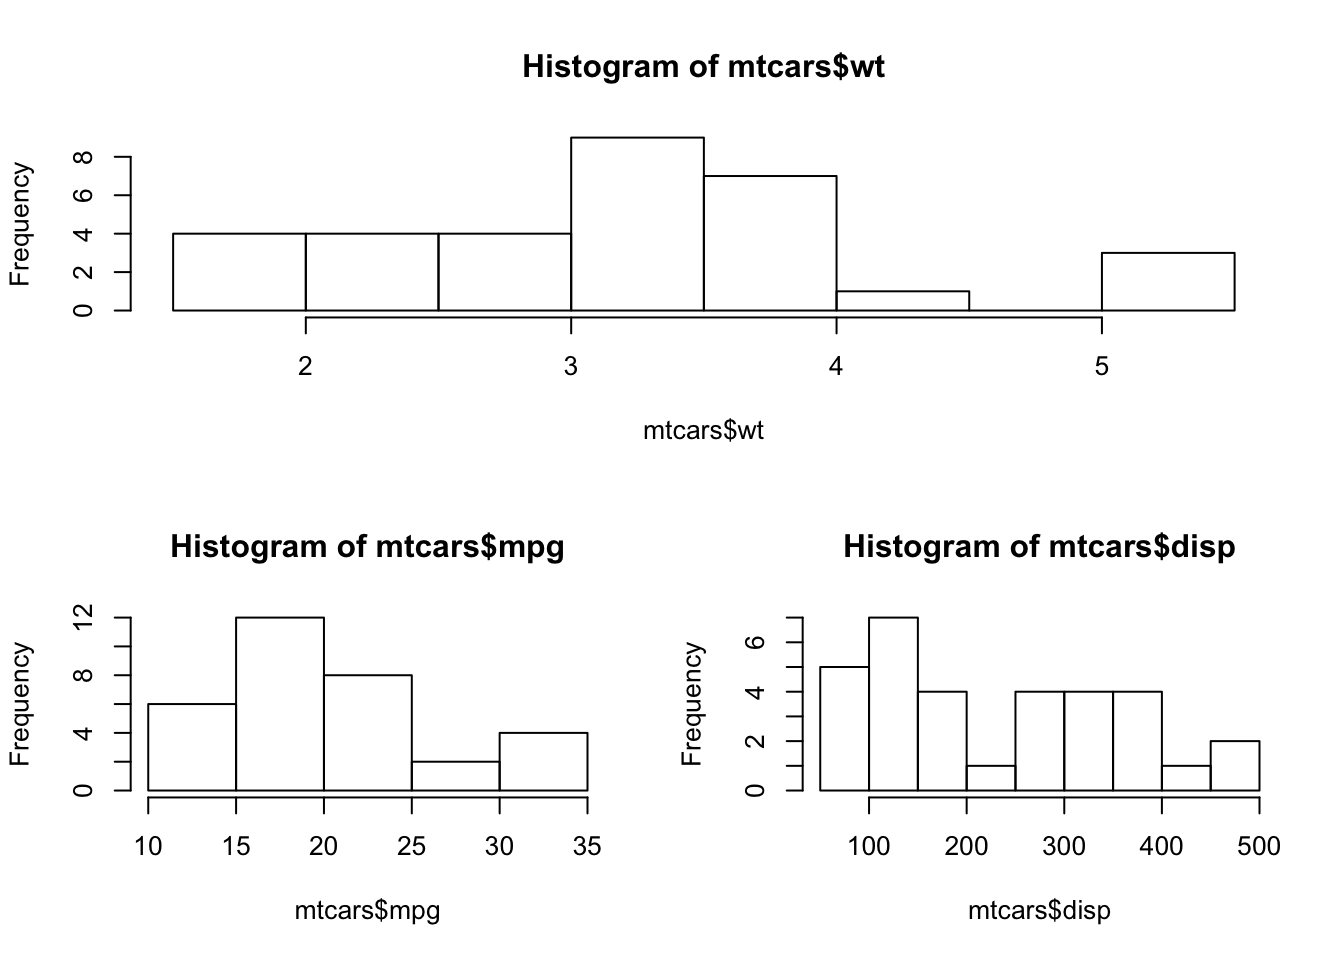
\includegraphics{R_notes_files/figure-latex/unnamed-chunk-4-1.pdf}

geom\_point() creates a scatter plot on top of the empty base. `mapping'
is an argument you beed to define. It maps variable to a way to show it
on graph or `defines how variables in your dataset are mapped to visual
properties'.

Mapping is always paired with aes() and the x and y arguments of aes(),
which specify which variable is x and which one is y.

\begin{Shaded}
\begin{Highlighting}[]
\KeywordTok{ggplot}\NormalTok{(}\DataTypeTok{data =}\NormalTok{ mpg) }\OperatorTok{+}\StringTok{ }
\StringTok{  }\KeywordTok{geom_point}\NormalTok{(}\DataTypeTok{mapping =} \KeywordTok{aes}\NormalTok{(}\DataTypeTok{x =}\NormalTok{ displ, }\DataTypeTok{y =}\NormalTok{ hwy))}
\end{Highlighting}
\end{Shaded}

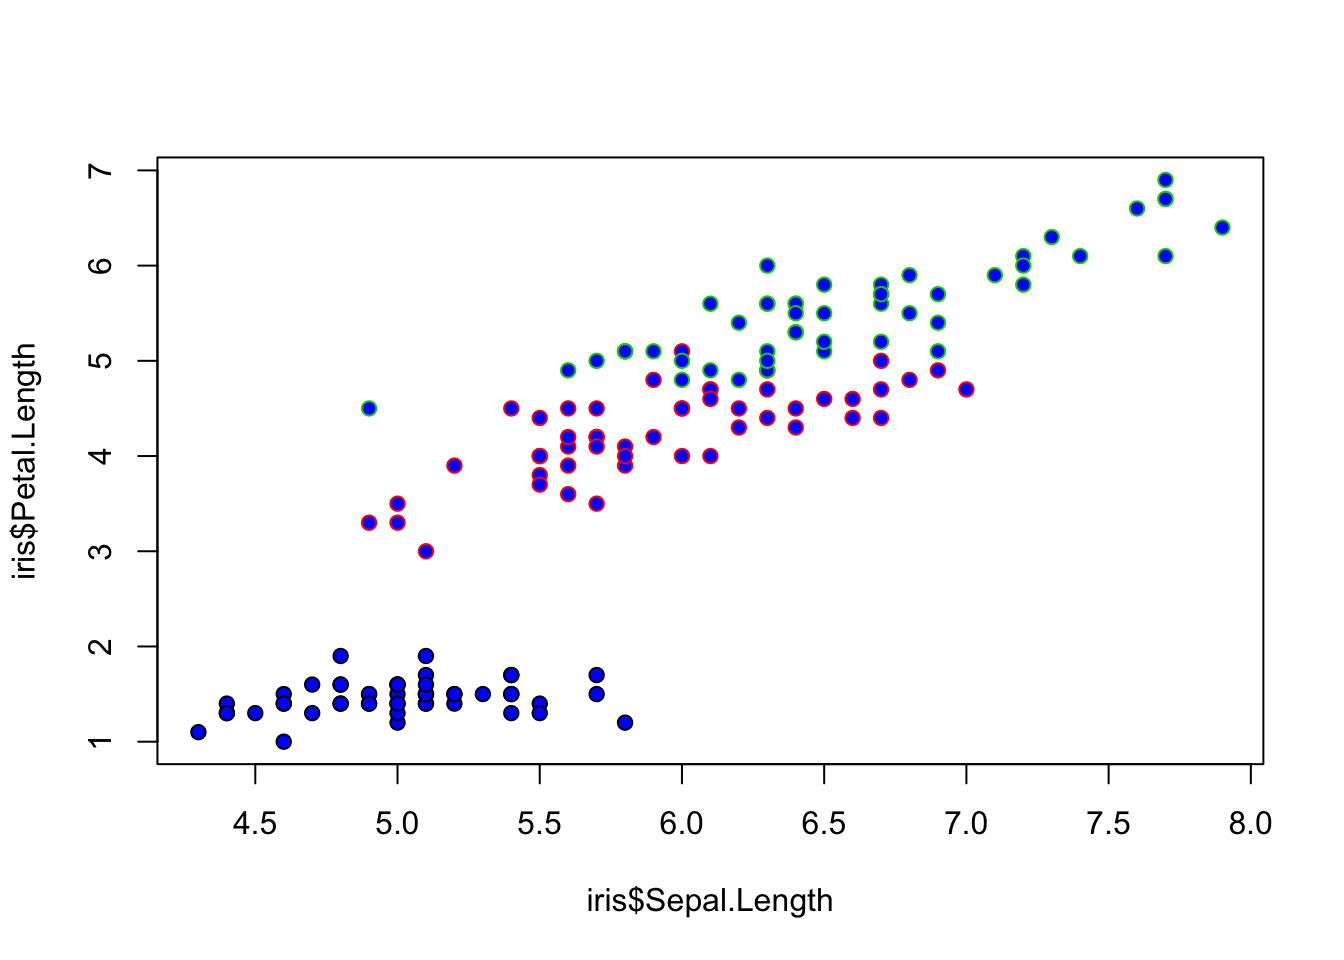
\includegraphics{R_notes_files/figure-latex/unnamed-chunk-5-1.pdf}

\subsection{Aesthetics}\label{aesthetics}

The specific \texttt{mapping\ =\ aes()} options vary depending on the
type of geom. For geom\_point, the following mapping options are
available:

\begin{itemize}
\tightlist
\item
  colour - colour of the points.
\item
  size - where each dot will be different sizes depending on the class
  it belongs to. You can also control the min and max range of point
  sizes with:
  \texttt{scale\_size\_continuous/discrete(range\ =\ c(2,4))} -
  depending on whether the variable is continuous or discrete.
\item
  alpha - transparency of points.
\item
  shape - shape of the points. ggplot2 will only use 6 shapes at a time.
  By default additional groups will be unplotted
\end{itemize}

A different variable can be mapped to each of these aesthetics. ggplot
selects a reasonable scale and constructs a legend.

(The dataset \texttt{mpg} will be used in this section)

Here colour is mapped to the variable (column) class.

\begin{Shaded}
\begin{Highlighting}[]
\KeywordTok{ggplot}\NormalTok{(}\DataTypeTok{data =}\NormalTok{ mpg) }\OperatorTok{+}\StringTok{ }
\StringTok{  }\KeywordTok{geom_point}\NormalTok{(}\DataTypeTok{mapping =} \KeywordTok{aes}\NormalTok{(}\DataTypeTok{x =}\NormalTok{ displ, }\DataTypeTok{y =}\NormalTok{ hwy, }\DataTypeTok{colour =}\NormalTok{ class))}
\end{Highlighting}
\end{Shaded}

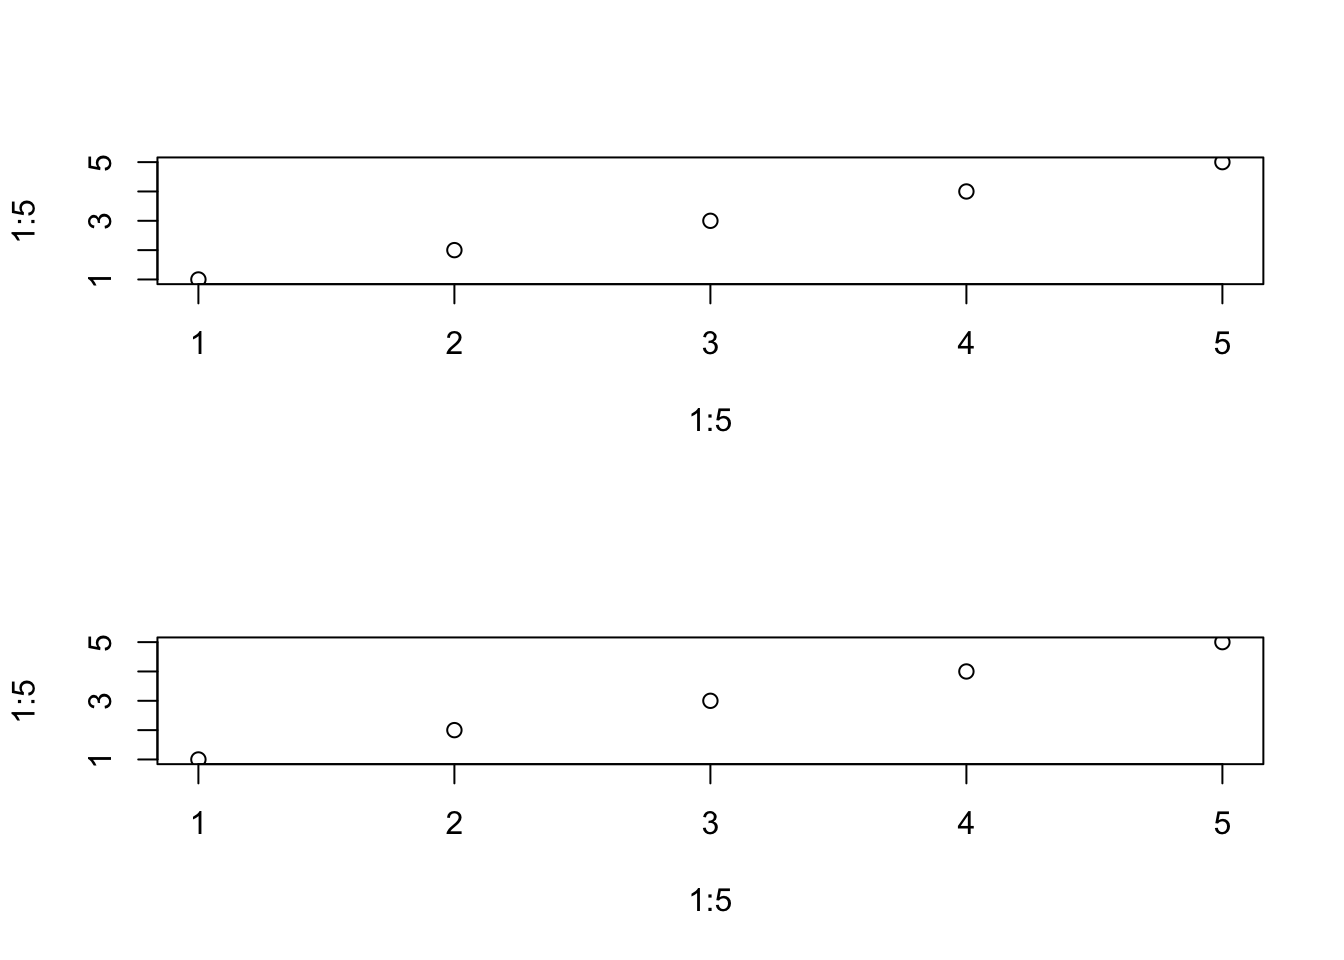
\includegraphics{R_notes_files/figure-latex/unnamed-chunk-6-1.pdf}

You can also set aesthetics manually. Do this by mapping aesthetic name
outside of the aes() function.

This makes all the points blue:

\begin{Shaded}
\begin{Highlighting}[]
\KeywordTok{ggplot}\NormalTok{(}\DataTypeTok{data =}\NormalTok{ mpg) }\OperatorTok{+}\StringTok{ }
\StringTok{  }\KeywordTok{geom_point}\NormalTok{(}\DataTypeTok{mapping =} \KeywordTok{aes}\NormalTok{(}\DataTypeTok{x =}\NormalTok{ displ, }\DataTypeTok{y =}\NormalTok{ hwy), }\DataTypeTok{colour =} \StringTok{"blue"}\NormalTok{)}
\end{Highlighting}
\end{Shaded}

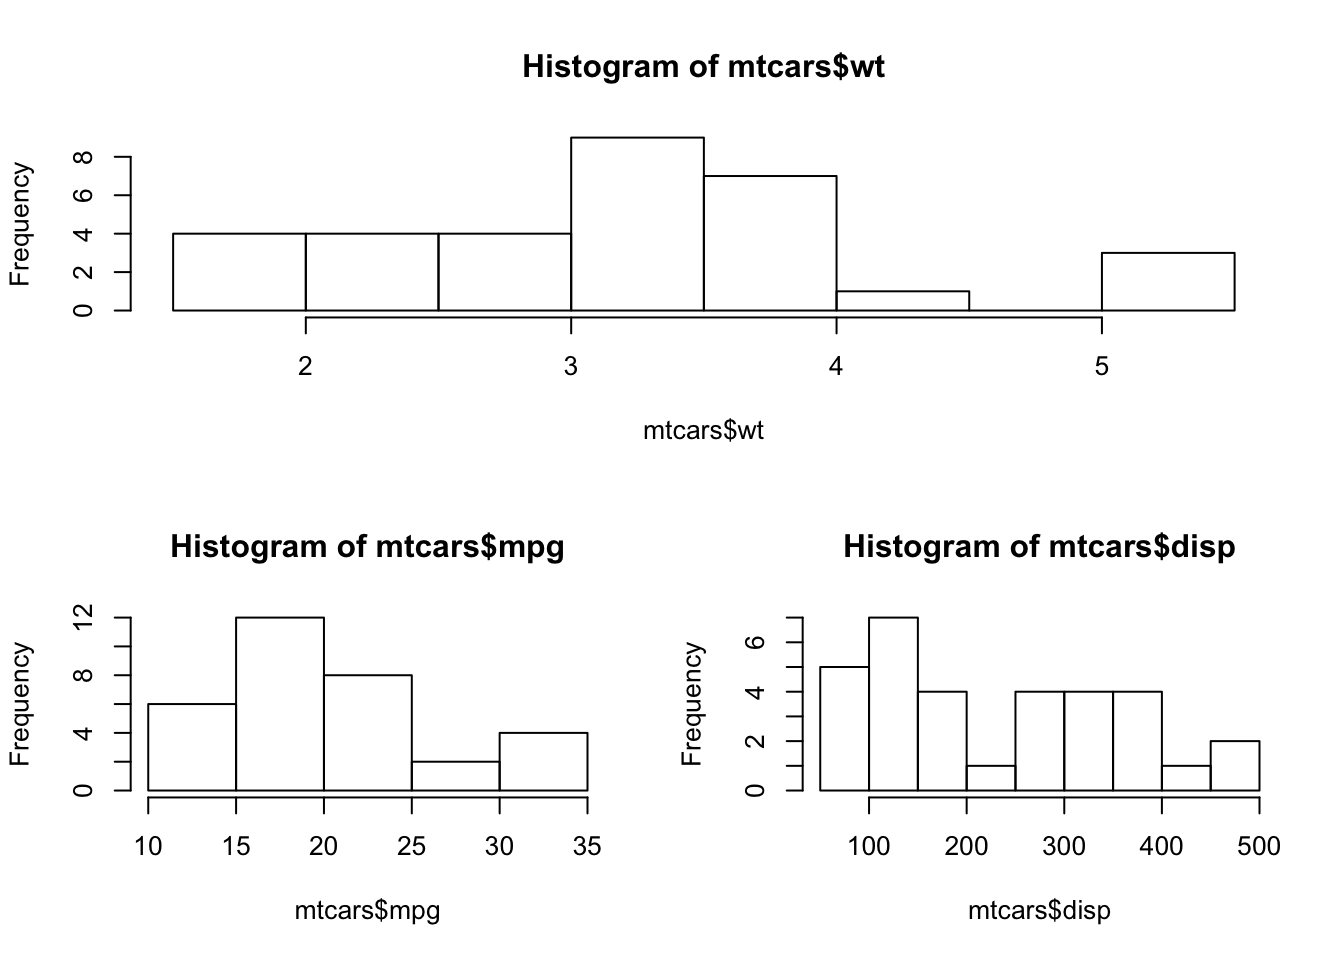
\includegraphics{R_notes_files/figure-latex/unnamed-chunk-7-1.pdf}

\begin{itemize}
\tightlist
\item
  size - you can specify size of all points in mm
\item
  shape - specify using a number code. The shapes available are:
  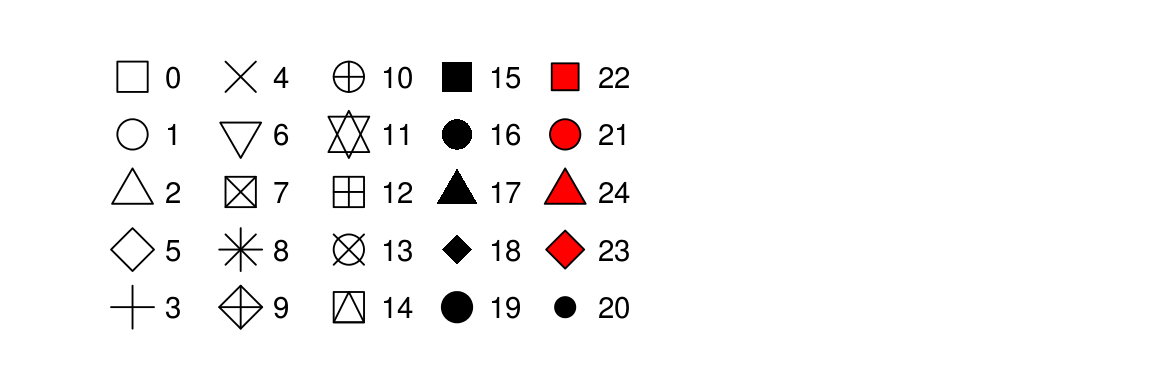
\includegraphics{Images/shapes-1.png}
\item
  stroke - for shapes that have a border, this dictates the size of the
  border, in mm.
\end{itemize}

Here we add a border to all the points:

\begin{Shaded}
\begin{Highlighting}[]
\KeywordTok{ggplot}\NormalTok{(}\DataTypeTok{data =}\NormalTok{ mpg, }\DataTypeTok{mapping =} \KeywordTok{aes}\NormalTok{(}\DataTypeTok{x =}\NormalTok{ displ, }\DataTypeTok{y =}\NormalTok{ hwy)) }\OperatorTok{+}
\StringTok{  }\KeywordTok{geom_point}\NormalTok{(}\DataTypeTok{colour =} \StringTok{"black"}\NormalTok{, }\DataTypeTok{shape =} \DecValTok{21}\NormalTok{, }\DataTypeTok{stroke =} \DecValTok{1}\NormalTok{, }\DataTypeTok{size =} \DecValTok{4}\NormalTok{, }
             \KeywordTok{aes}\NormalTok{(}\DataTypeTok{fill =} \KeywordTok{factor}\NormalTok{(drv)))}
\end{Highlighting}
\end{Shaded}

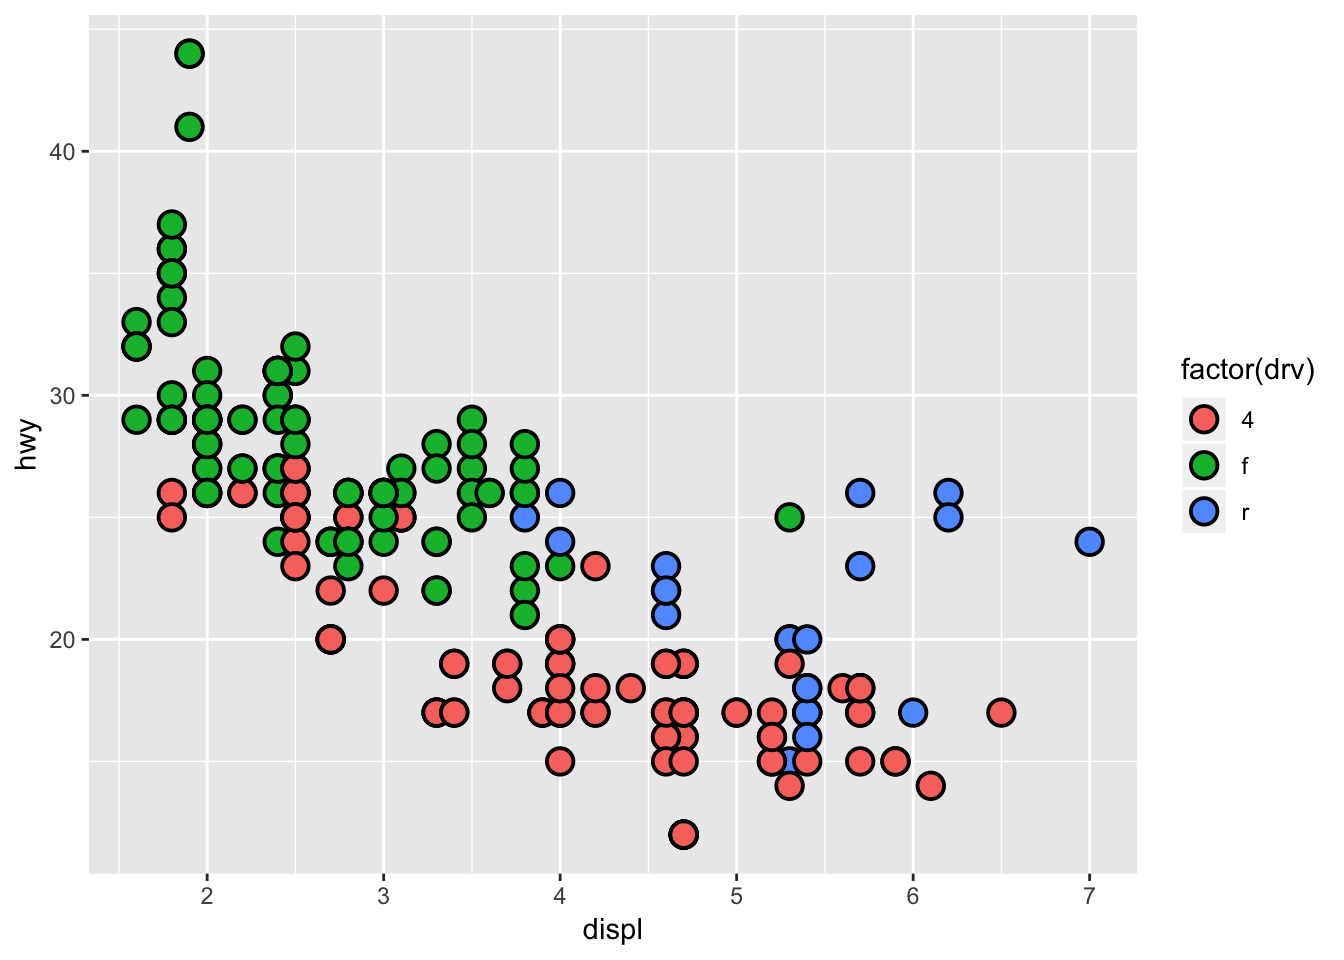
\includegraphics{R_notes_files/figure-latex/unnamed-chunk-8-1.pdf}

\subsection{Syntax}\label{syntax}

If you put mappings at the top in ggplot(), it will use such mapping for
everything, `global mapping'.

Here the same y and x mappings are used to create points and a smooth
line.

\begin{Shaded}
\begin{Highlighting}[]
\KeywordTok{ggplot}\NormalTok{(}\DataTypeTok{data =}\NormalTok{ mpg, }\DataTypeTok{mapping =} \KeywordTok{aes}\NormalTok{(}\DataTypeTok{x =}\NormalTok{ displ, }\DataTypeTok{y =}\NormalTok{ hwy)) }\OperatorTok{+}\StringTok{ }
\StringTok{  }\KeywordTok{geom_point}\NormalTok{() }\OperatorTok{+}\StringTok{ }
\StringTok{  }\KeywordTok{geom_smooth}\NormalTok{()}
\end{Highlighting}
\end{Shaded}

\begin{verbatim}
## `geom_smooth()` using method = 'loess' and formula 'y ~ x'
\end{verbatim}

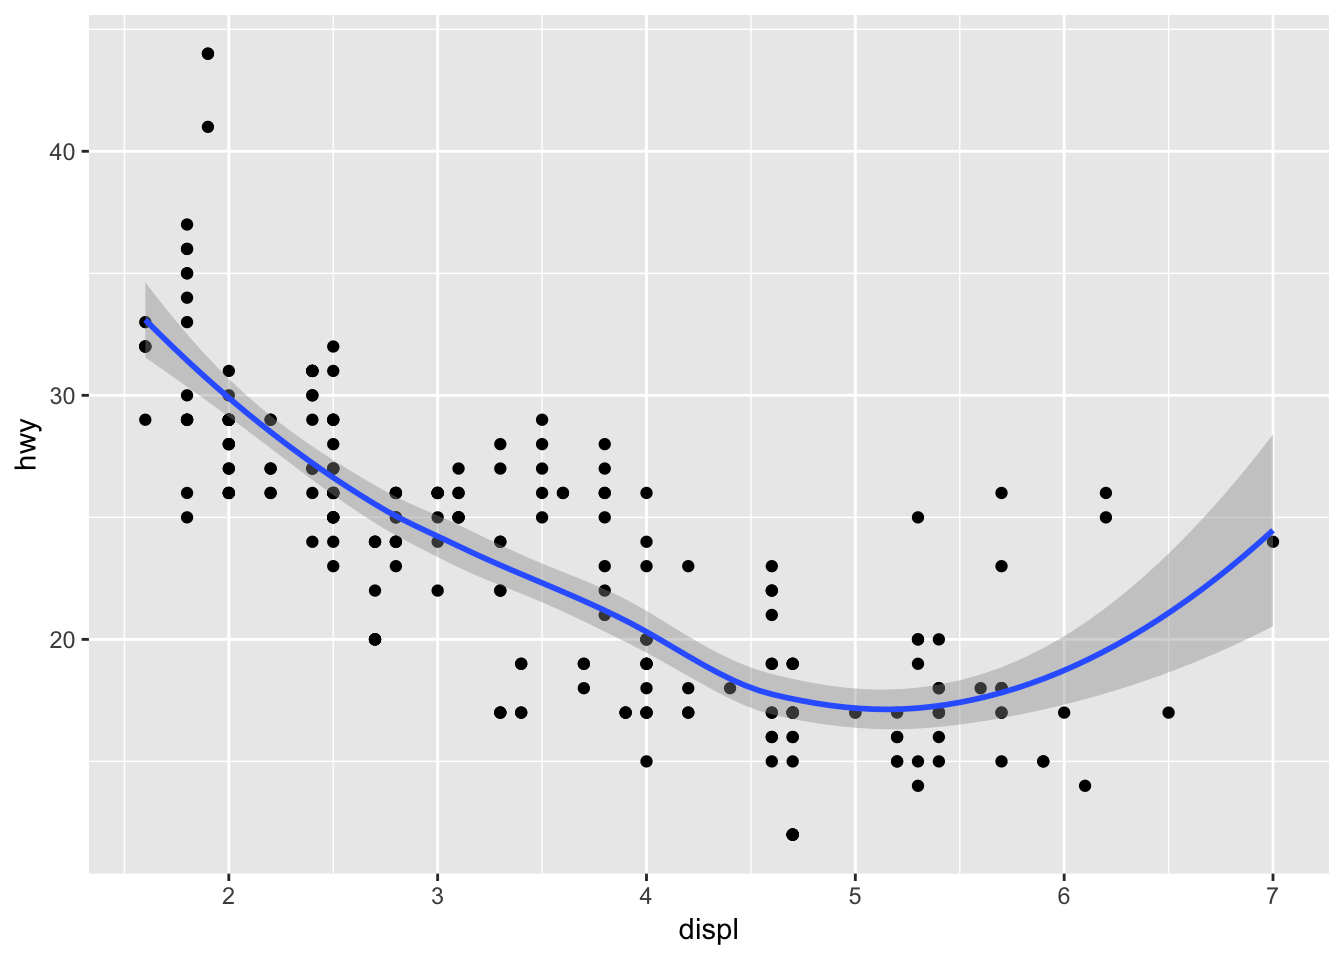
\includegraphics{R_notes_files/figure-latex/unnamed-chunk-9-1.pdf}

The above code means the same as:

\begin{Shaded}
\begin{Highlighting}[]
\KeywordTok{ggplot}\NormalTok{(}\DataTypeTok{data =}\NormalTok{ mpg) }\OperatorTok{+}\StringTok{ }
\StringTok{  }\KeywordTok{geom_point}\NormalTok{(}\DataTypeTok{mapping =} \KeywordTok{aes}\NormalTok{(}\DataTypeTok{x =}\NormalTok{ displ, }\DataTypeTok{y =}\NormalTok{ hwy)) }\OperatorTok{+}
\StringTok{  }\KeywordTok{geom_smooth}\NormalTok{(}\DataTypeTok{mapping =} \KeywordTok{aes}\NormalTok{(}\DataTypeTok{x =}\NormalTok{ displ, }\DataTypeTok{y =}\NormalTok{ hwy))}
\end{Highlighting}
\end{Shaded}

You can still change mappings for specific geoms, even if you have
specified a `global' mapping in \texttt{ggplot()} call. If you add
mappings to \texttt{geom\_xx()}, ggplot2 will overwrite or extend the
global mappings given in ggplot() with the local mappings given in
geom\_xx(). Again we can consider geom() as another layer underneath
ggplot(), and any changes are for the layer geom(). Here, we add the
colour variable to just the \texttt{geom\_point()} layer.

\begin{Shaded}
\begin{Highlighting}[]
\KeywordTok{ggplot}\NormalTok{(}\DataTypeTok{data =}\NormalTok{ mpg, }\DataTypeTok{mapping =} \KeywordTok{aes}\NormalTok{(}\DataTypeTok{x =}\NormalTok{ displ, }\DataTypeTok{y =}\NormalTok{ hwy)) }\OperatorTok{+}\StringTok{ }
\StringTok{  }\KeywordTok{geom_point}\NormalTok{(}\DataTypeTok{mapping =} \KeywordTok{aes}\NormalTok{(}\DataTypeTok{color =}\NormalTok{ class)) }\OperatorTok{+}\StringTok{ }
\StringTok{  }\KeywordTok{geom_smooth}\NormalTok{()}
\end{Highlighting}
\end{Shaded}

\begin{verbatim}
## `geom_smooth()` using method = 'loess' and formula 'y ~ x'
\end{verbatim}

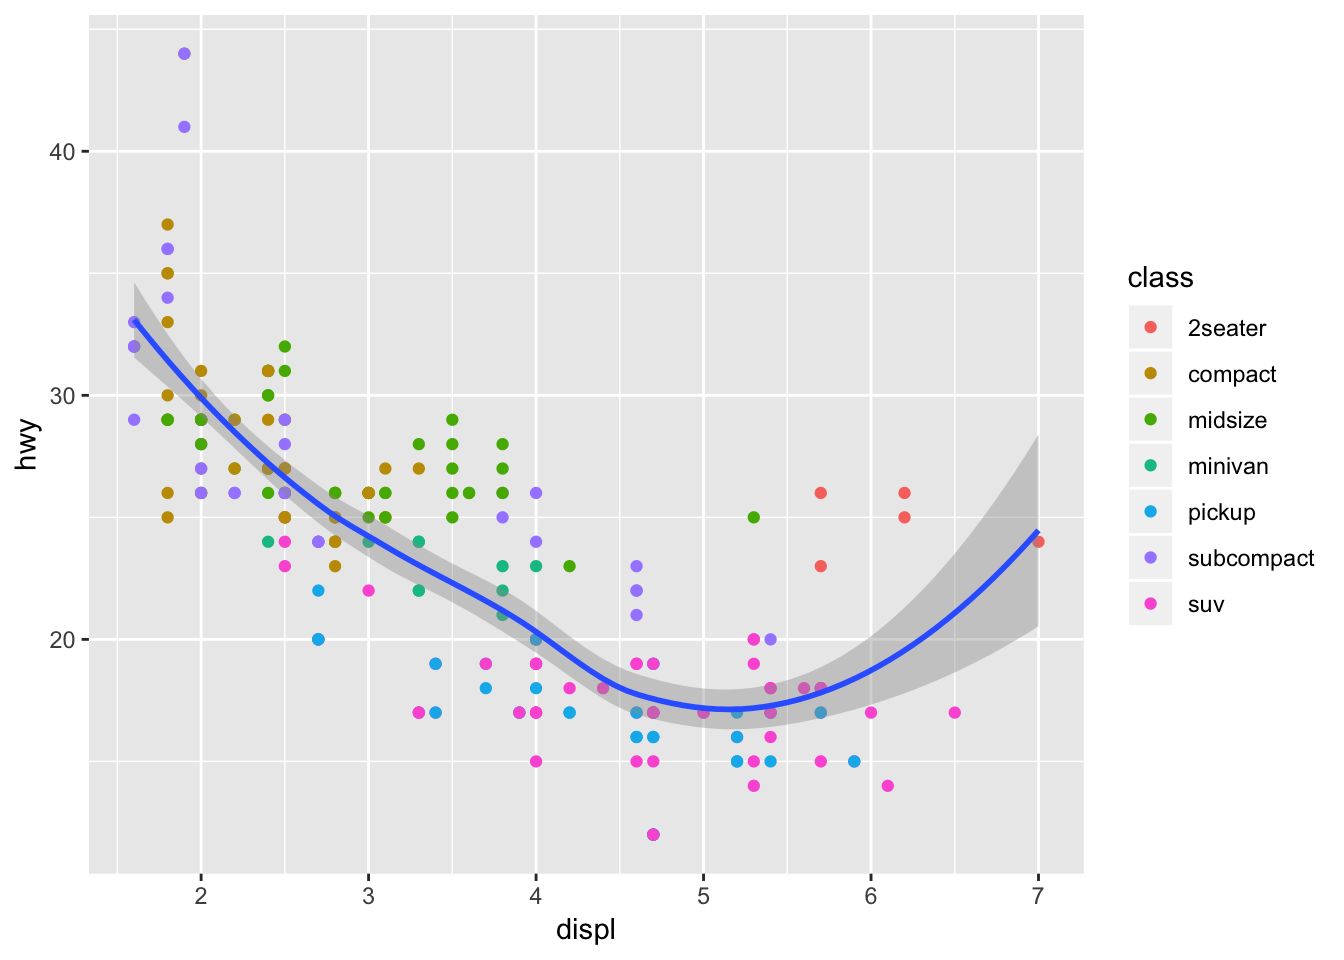
\includegraphics{R_notes_files/figure-latex/unnamed-chunk-11-1.pdf}

You can also simplify the syntax as \texttt{data\ =} and
\texttt{mapping\ =} are the first arguments to the \texttt{ggplot()} and
\texttt{geom\_xx()} functions.

\subsection{Stat}\label{stat}

Stat stands for statistical transform and is the algorithm used by a
geom to calculate the values used for the graphs. You can find the
default stat by looking in the help file of that geom.

You can use stat and geom interchangeably. For example, the default stat
for \texttt{geom\_bar()} is \texttt{stat\_count()}.

\begin{Shaded}
\begin{Highlighting}[]
\CommentTok{# this code:}
\KeywordTok{ggplot}\NormalTok{(iris) }\OperatorTok{+}\StringTok{ }
\StringTok{  }\KeywordTok{stat_count}\NormalTok{(}\KeywordTok{aes}\NormalTok{(}\DataTypeTok{x =}\NormalTok{ Species))}

\CommentTok{# is the same as:}
\KeywordTok{ggplot}\NormalTok{(iris) }\OperatorTok{+}\StringTok{ }
\StringTok{  }\KeywordTok{geom_bar}\NormalTok{(}\KeywordTok{aes}\NormalTok{(}\DataTypeTok{x =}\NormalTok{ Species))}
\end{Highlighting}
\end{Shaded}

The help file for \texttt{geom\_bar()} will also document what values
are computed for this stat. \texttt{stat\_count()} computes 2 values:
count and prop.

You can override the default stat with the \texttt{stat} argument in
\texttt{geom\_xx()}. You can also change the default mapping e.g.~so
that a bar graph of proportion is shown instead of counts.

\begin{Shaded}
\begin{Highlighting}[]
\KeywordTok{ggplot}\NormalTok{(iris) }\OperatorTok{+}\StringTok{ }
\StringTok{  }\KeywordTok{geom_bar}\NormalTok{(}\KeywordTok{aes}\NormalTok{(}\DataTypeTok{x =}\NormalTok{ Species, }\DataTypeTok{y =}\NormalTok{ ..prop.., }\DataTypeTok{group =} \DecValTok{1}\NormalTok{))}
\end{Highlighting}
\end{Shaded}

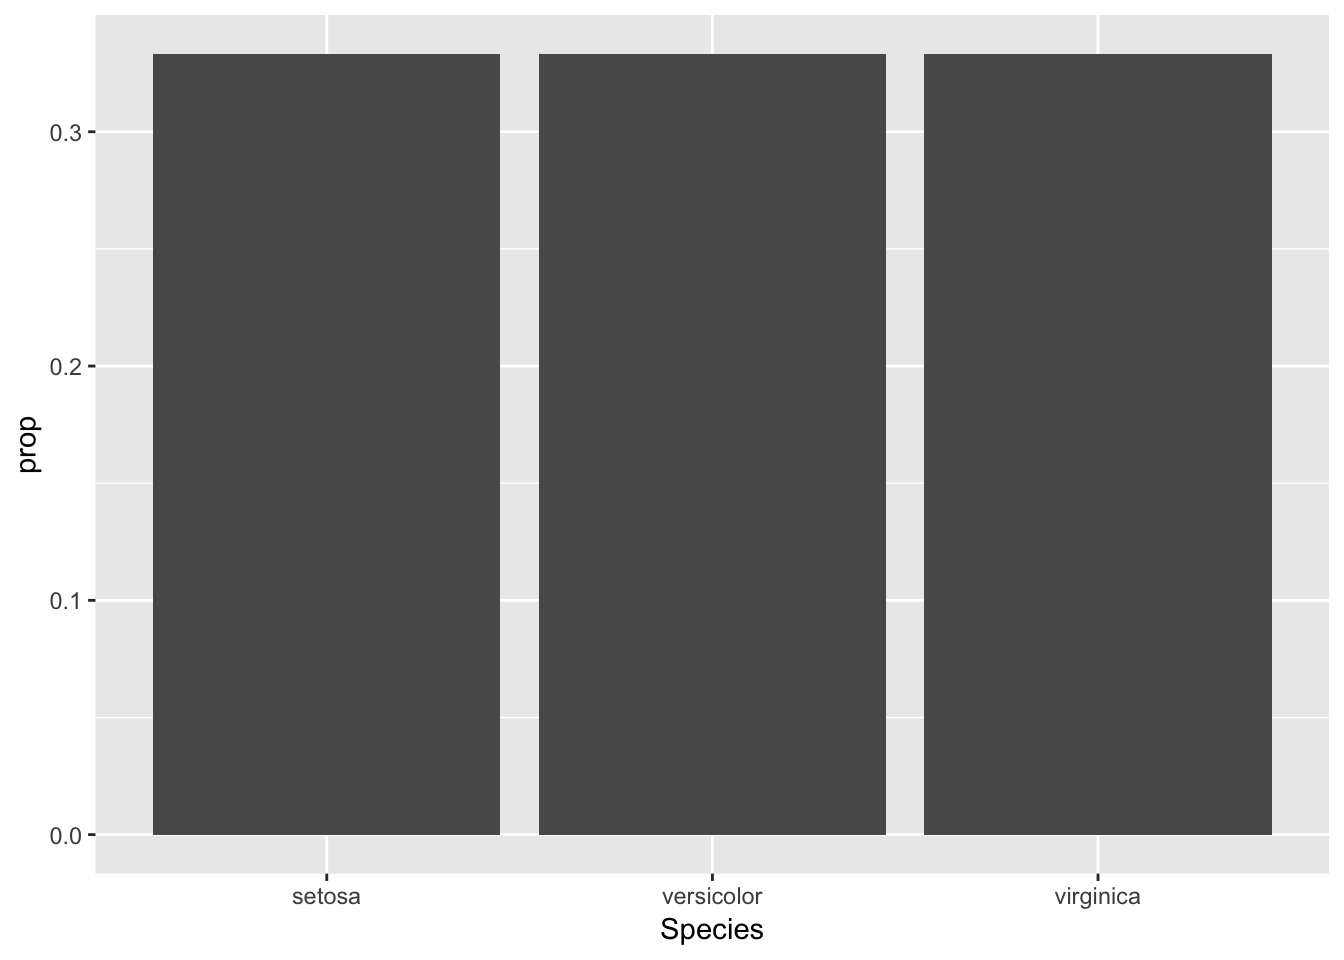
\includegraphics{R_notes_files/figure-latex/unnamed-chunk-13-1.pdf}

Note that proportion is now on the y axis. The argument
\texttt{group\ =\ 1} means that it will treat all observations as 100\%
and calculated the proportion of observations in each group. Without
this argument, the proportion will be 100\% for each group as it will
treat each group separately.

\section{geom\_point}\label{geom_point}

The \texttt{iris} dataset will be used for this section.

\subsection{Jitter}\label{jitter}

A problem with scatter plots is that if there are many values that are
the same number (especially if they are rounded), the points will
overlap each other and it will be diff to appreciate from the graph
where the weight of the points lie. To overcome this you can separate
the points by adding a bit of random noise to each point. You can do
this in two ways:

\begin{Shaded}
\begin{Highlighting}[]
\KeywordTok{ggplot}\NormalTok{(}\DataTypeTok{data =}\NormalTok{ mpg) }\OperatorTok{+}\StringTok{ }
\StringTok{  }\KeywordTok{geom_point}\NormalTok{(}\DataTypeTok{mapping =} \KeywordTok{aes}\NormalTok{(}\DataTypeTok{x =}\NormalTok{ displ, }\DataTypeTok{y =}\NormalTok{ hwy), }\DataTypeTok{position =} \StringTok{"jitter"}\NormalTok{)}
\end{Highlighting}
\end{Shaded}

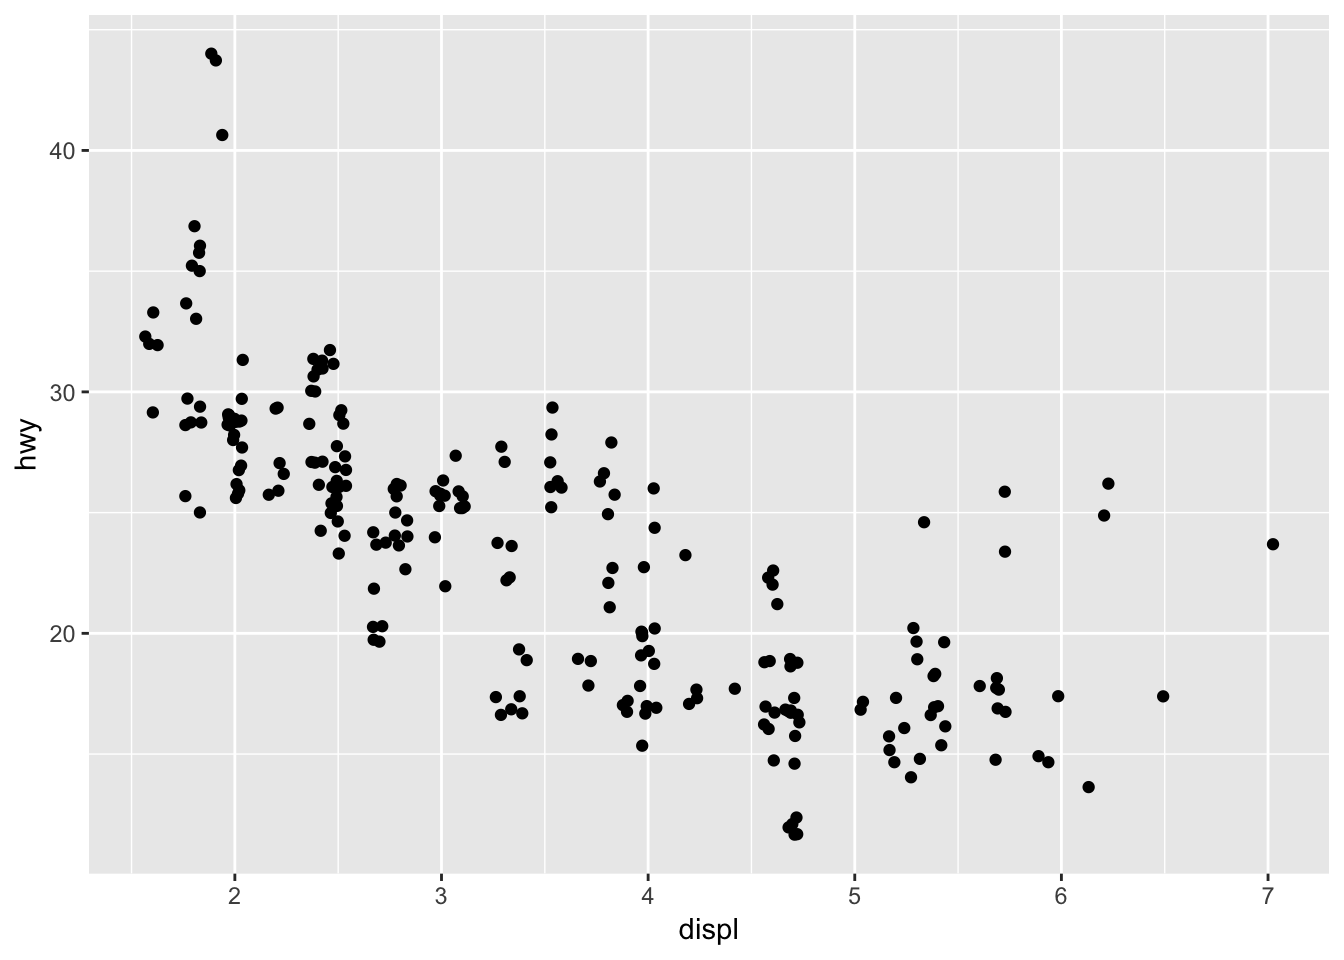
\includegraphics{R_notes_files/figure-latex/unnamed-chunk-14-1.pdf}

or in a shorter way (as \texttt{geom\_point(position\ =\ "jitter")} =
\texttt{geom\_jitter()}):

\begin{Shaded}
\begin{Highlighting}[]
\KeywordTok{ggplot}\NormalTok{(mpg) }\OperatorTok{+}\StringTok{ }
\StringTok{  }\KeywordTok{geom_jitter}\NormalTok{(}\KeywordTok{aes}\NormalTok{(}\DataTypeTok{x =}\NormalTok{ displ, }\DataTypeTok{y =}\NormalTok{ hwy))}
\end{Highlighting}
\end{Shaded}

\subsection{Labels}\label{labels}

To label points, use \texttt{geom\_text}:

\begin{Shaded}
\begin{Highlighting}[]
\KeywordTok{ggplot}\NormalTok{(iris, }\KeywordTok{aes}\NormalTok{(}\DataTypeTok{y =}\NormalTok{ Petal.Width, }\DataTypeTok{x =}\NormalTok{ Petal.Length)) }\OperatorTok{+}\StringTok{ }
\StringTok{  }\KeywordTok{geom_point}\NormalTok{() }\OperatorTok{+}\StringTok{ }
\StringTok{  }\KeywordTok{geom_text}\NormalTok{(}\KeywordTok{aes}\NormalTok{(}\DataTypeTok{label =}\NormalTok{ iris}\OperatorTok{$}\NormalTok{Species))}
\end{Highlighting}
\end{Shaded}

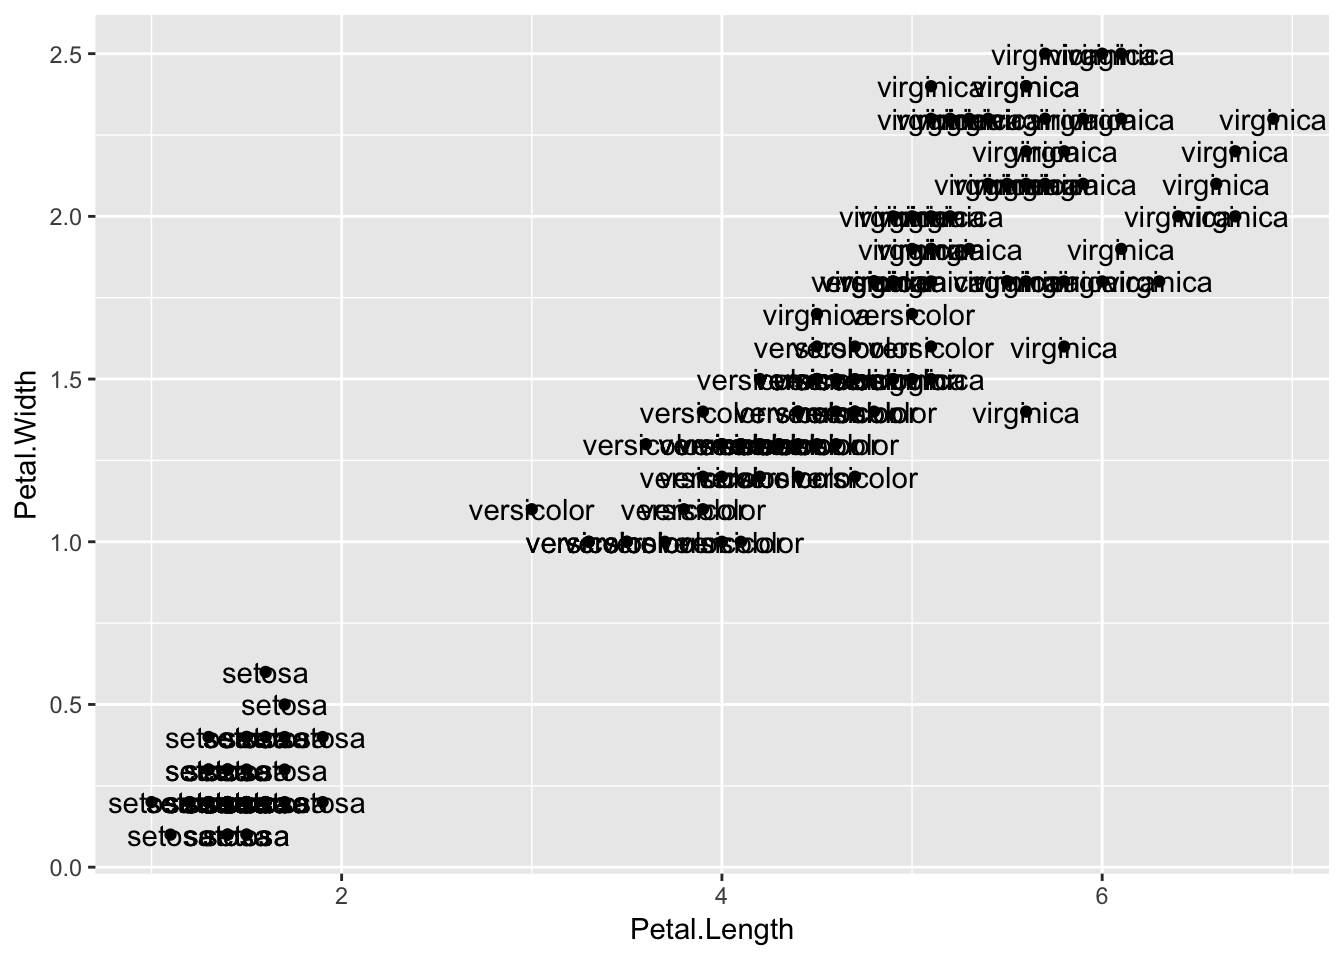
\includegraphics{R_notes_files/figure-latex/unnamed-chunk-16-1.pdf}

If you only wanted to label a few specific points, you can use
\texttt{ifelse()}:

\begin{Shaded}
\begin{Highlighting}[]
\KeywordTok{ggplot}\NormalTok{(iris, }\KeywordTok{aes}\NormalTok{(}\DataTypeTok{y =}\NormalTok{ Petal.Width, }\DataTypeTok{x =}\NormalTok{ Petal.Length)) }\OperatorTok{+}\StringTok{ }
\StringTok{  }\KeywordTok{geom_point}\NormalTok{() }\OperatorTok{+}\StringTok{ }
\StringTok{  }\KeywordTok{geom_text}\NormalTok{(}\KeywordTok{aes}\NormalTok{(}\DataTypeTok{label =} \KeywordTok{ifelse}\NormalTok{(iris}\OperatorTok{$}\NormalTok{Petal.Length }\OperatorTok{>}\StringTok{ }\FloatTok{6.2}\NormalTok{, }
                               \KeywordTok{as.character}\NormalTok{(iris}\OperatorTok{$}\NormalTok{Species), }\StringTok{""}\NormalTok{)), }
            \DataTypeTok{hjust =} \FloatTok{0.5}\NormalTok{, }\DataTypeTok{vjust =} \DecValTok{1}\NormalTok{)}
\end{Highlighting}
\end{Shaded}

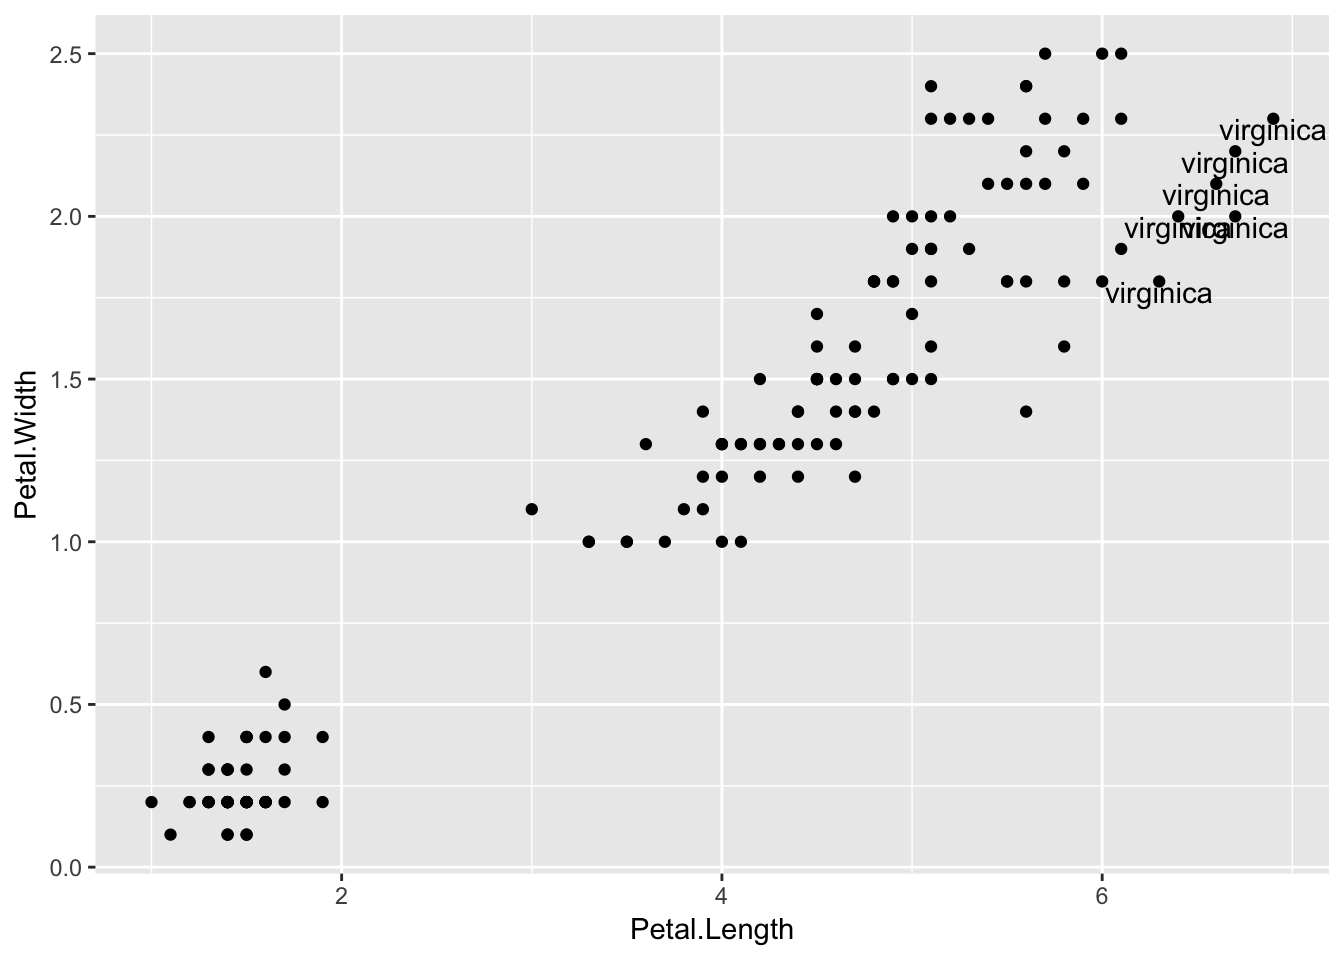
\includegraphics{R_notes_files/figure-latex/unnamed-chunk-17-1.pdf}

Note that in the \texttt{ifelse()} statement, you specify the label to
be empty \texttt{""} if the value (row) does not meet your condition.

The arguments \texttt{hjust} and \texttt{vjust} change the position of
the label. Note that these are arguments to \texttt{geom\_text()} and
not \texttt{aes()}.

Overlapping labels is a common problem. The package \texttt{ggrepel} (
\href{https://cran.r-project.org/web/packages/ggrepel/vignettes/ggrepel.html}{link}
) solves this problem.

\begin{Shaded}
\begin{Highlighting}[]
\KeywordTok{library}\NormalTok{(ggrepel)}

\KeywordTok{ggplot}\NormalTok{(iris, }\KeywordTok{aes}\NormalTok{(}\DataTypeTok{y =}\NormalTok{ Petal.Width, }\DataTypeTok{x =}\NormalTok{ Petal.Length)) }\OperatorTok{+}\StringTok{ }
\StringTok{  }\KeywordTok{geom_point}\NormalTok{() }\OperatorTok{+}\StringTok{ }
\StringTok{  }\KeywordTok{geom_text_repel}\NormalTok{(}\KeywordTok{aes}\NormalTok{(}\DataTypeTok{label =} \KeywordTok{ifelse}\NormalTok{(iris}\OperatorTok{$}\NormalTok{Petal.Length }\OperatorTok{>}\StringTok{ }\FloatTok{6.2}\NormalTok{,}
                                     \KeywordTok{as.character}\NormalTok{(iris}\OperatorTok{$}\NormalTok{Species), }\StringTok{""}\NormalTok{)))}
\end{Highlighting}
\end{Shaded}

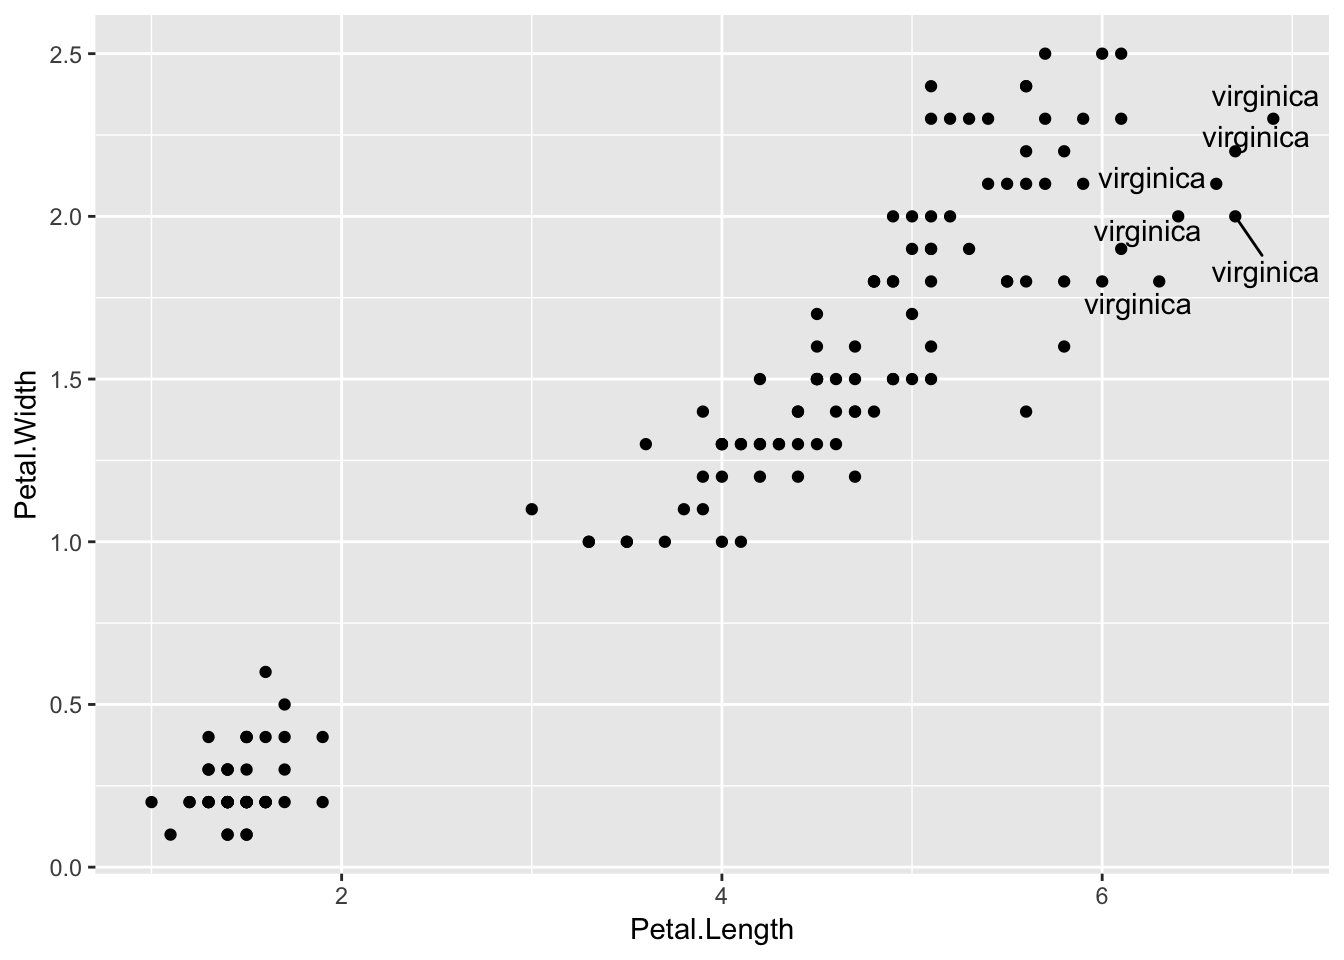
\includegraphics{R_notes_files/figure-latex/unnamed-chunk-18-1.pdf}

Note that you no longer use \texttt{geom\_text()}. We also put the label
argument within \texttt{geom\_text\_repel(aes())}. You can also the
\texttt{label} argument within ggplot, so it is set `globally'.

\subsection{Colour points}\label{colour-points}

If you use the aesthetic \texttt{fill} to colour points using a
categorical variable, ggplot2 will set different colours for each
category. If you use a continuous variable, ggplot2 will set a gradient
scale with appropriate min and max values.

To colour specific points you can use \texttt{cut()} with
\texttt{scale\_colour\_manual()}:

\begin{Shaded}
\begin{Highlighting}[]
\KeywordTok{ggplot}\NormalTok{(iris, }\KeywordTok{aes}\NormalTok{(}\DataTypeTok{y =}\NormalTok{ Petal.Width, }\DataTypeTok{x =}\NormalTok{ Petal.Length, }
                 \DataTypeTok{colour =} \KeywordTok{cut}\NormalTok{(iris}\OperatorTok{$}\NormalTok{Petal.Length, }\KeywordTok{c}\NormalTok{(}\DecValTok{0}\NormalTok{,}\DecValTok{6}\NormalTok{,}\DecValTok{10}\NormalTok{)))) }\OperatorTok{+}\StringTok{ }
\StringTok{  }\KeywordTok{geom_point}\NormalTok{() }\OperatorTok{+}
\StringTok{  }\KeywordTok{scale_colour_manual}\NormalTok{(}\DataTypeTok{name =} \StringTok{"legend"}\NormalTok{, }\DataTypeTok{values =} \KeywordTok{c}\NormalTok{(}\StringTok{"red"}\NormalTok{, }\StringTok{"black"}\NormalTok{))}
\end{Highlighting}
\end{Shaded}

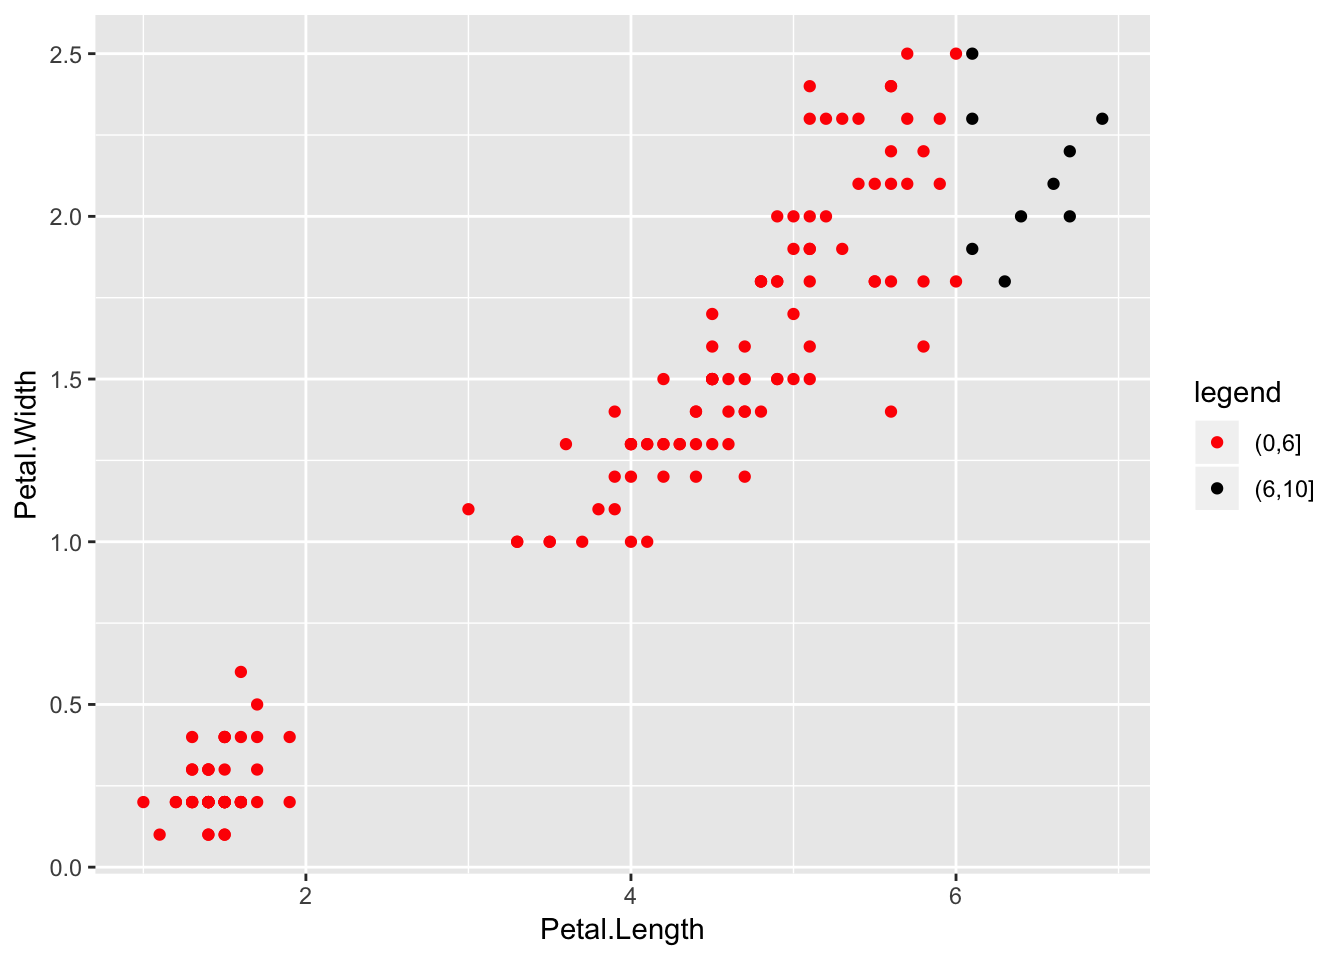
\includegraphics{R_notes_files/figure-latex/unnamed-chunk-19-1.pdf}

The function \texttt{cut()} divides a vector into intervals. You can
either specify break points (as I have above - note providing 3 numbers
breaks the vector into 2 intervals) or specify the number of intervals
you want, in the \texttt{breaks} argument. The result is a factor, where
each level is an interval.

The \texttt{scale\_colour\_manual()} function lets you specify which
colours you wish to use. You can also modify the legend by changing the
name and the legend labels.

Here we will change the legend labels:

\begin{Shaded}
\begin{Highlighting}[]
\KeywordTok{ggplot}\NormalTok{(iris, }\KeywordTok{aes}\NormalTok{(}\DataTypeTok{y =}\NormalTok{ Petal.Width, }\DataTypeTok{x =}\NormalTok{ Petal.Length, }
                 \DataTypeTok{colour =} \KeywordTok{cut}\NormalTok{(iris}\OperatorTok{$}\NormalTok{Petal.Length, }\KeywordTok{c}\NormalTok{(}\DecValTok{0}\NormalTok{,}\DecValTok{6}\NormalTok{,}\DecValTok{10}\NormalTok{)))) }\OperatorTok{+}\StringTok{ }
\StringTok{  }\KeywordTok{geom_point}\NormalTok{() }\OperatorTok{+}
\StringTok{  }\KeywordTok{scale_colour_manual}\NormalTok{(}\DataTypeTok{name =} \StringTok{"legend"}\NormalTok{, }\DataTypeTok{values =} \KeywordTok{c}\NormalTok{(}\StringTok{"red"}\NormalTok{, }\StringTok{"black"}\NormalTok{), }
                      \DataTypeTok{labels =} \KeywordTok{c}\NormalTok{(}\StringTok{"less than 6"}\NormalTok{, }\StringTok{"larger than 6"}\NormalTok{))}
\end{Highlighting}
\end{Shaded}

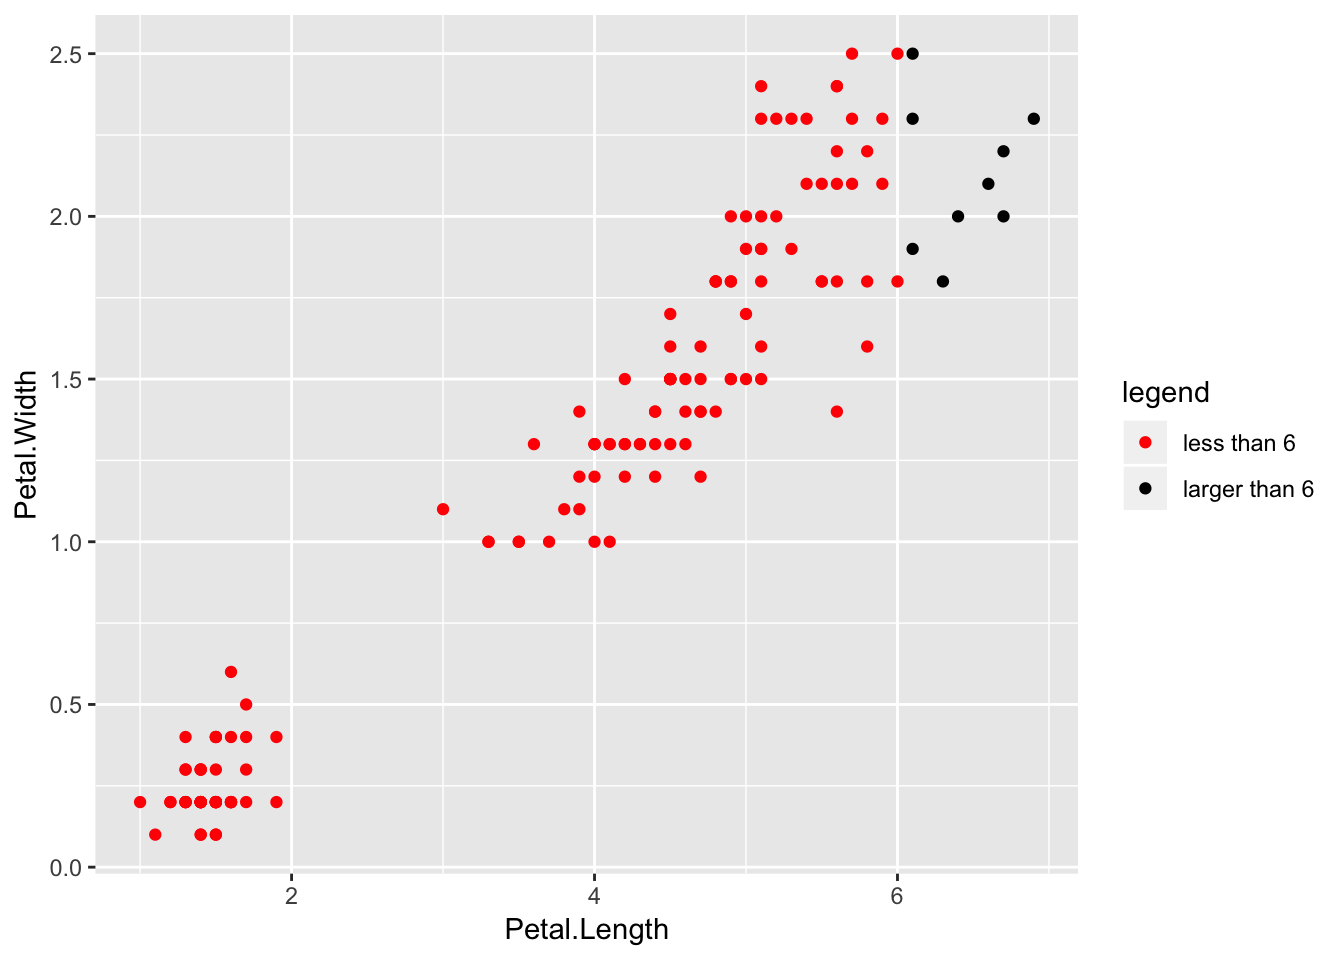
\includegraphics{R_notes_files/figure-latex/unnamed-chunk-20-1.pdf}

You can also do this by calling \texttt{geom\_point()} twice, specifying
only selected points in the second call and setting these points to be a
specific colour (see:
\href{https://stackoverflow.com/questions/11467965/r-ggplot2-highlighting-selected-points-and-strange-behavior}{SO}
).

\subsection{Matrix of plots}\label{matrix-of-plots}

Base R comes with the function \texttt{pairs()} which creates a matrix
of scatter plots.

\begin{Shaded}
\begin{Highlighting}[]
\KeywordTok{pairs}\NormalTok{(iris[,}\DecValTok{1}\OperatorTok{:}\DecValTok{4}\NormalTok{])}
\end{Highlighting}
\end{Shaded}

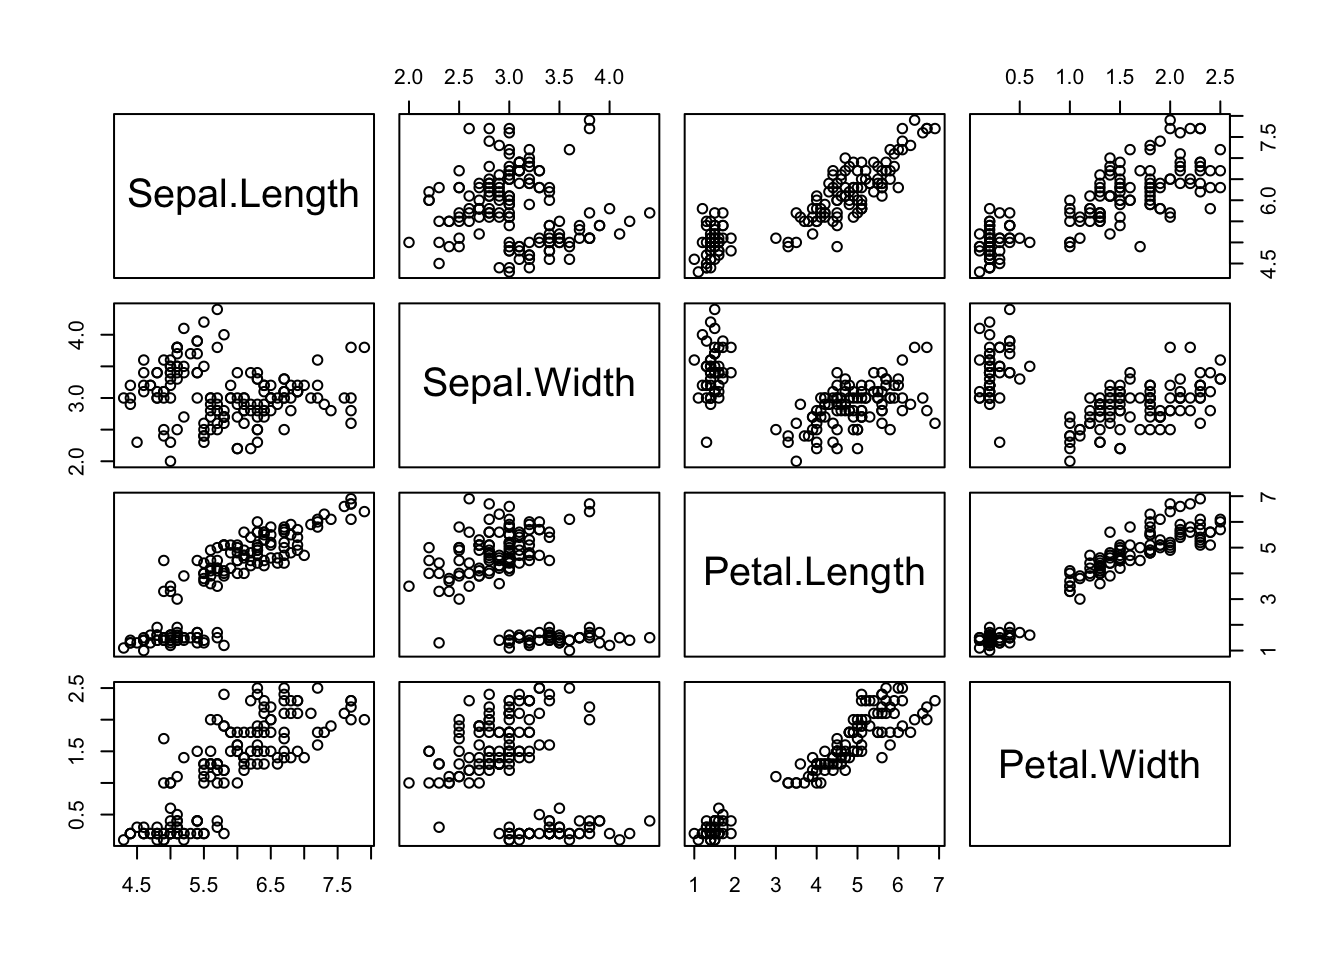
\includegraphics{R_notes_files/figure-latex/unnamed-chunk-21-1.pdf}

The \texttt{GGally} package is an extension to \texttt{ggplot2} and has
a function called \texttt{ggpairs()} which offers extra functionality,
like letting you use non-continuous variables in your data frames.

\begin{Shaded}
\begin{Highlighting}[]
\KeywordTok{library}\NormalTok{(GGally)}
\KeywordTok{ggpairs}\NormalTok{(iris, }\KeywordTok{aes}\NormalTok{(}\DataTypeTok{colour =}\NormalTok{ Species, }\DataTypeTok{alpha =} \FloatTok{0.4}\NormalTok{))}
\end{Highlighting}
\end{Shaded}

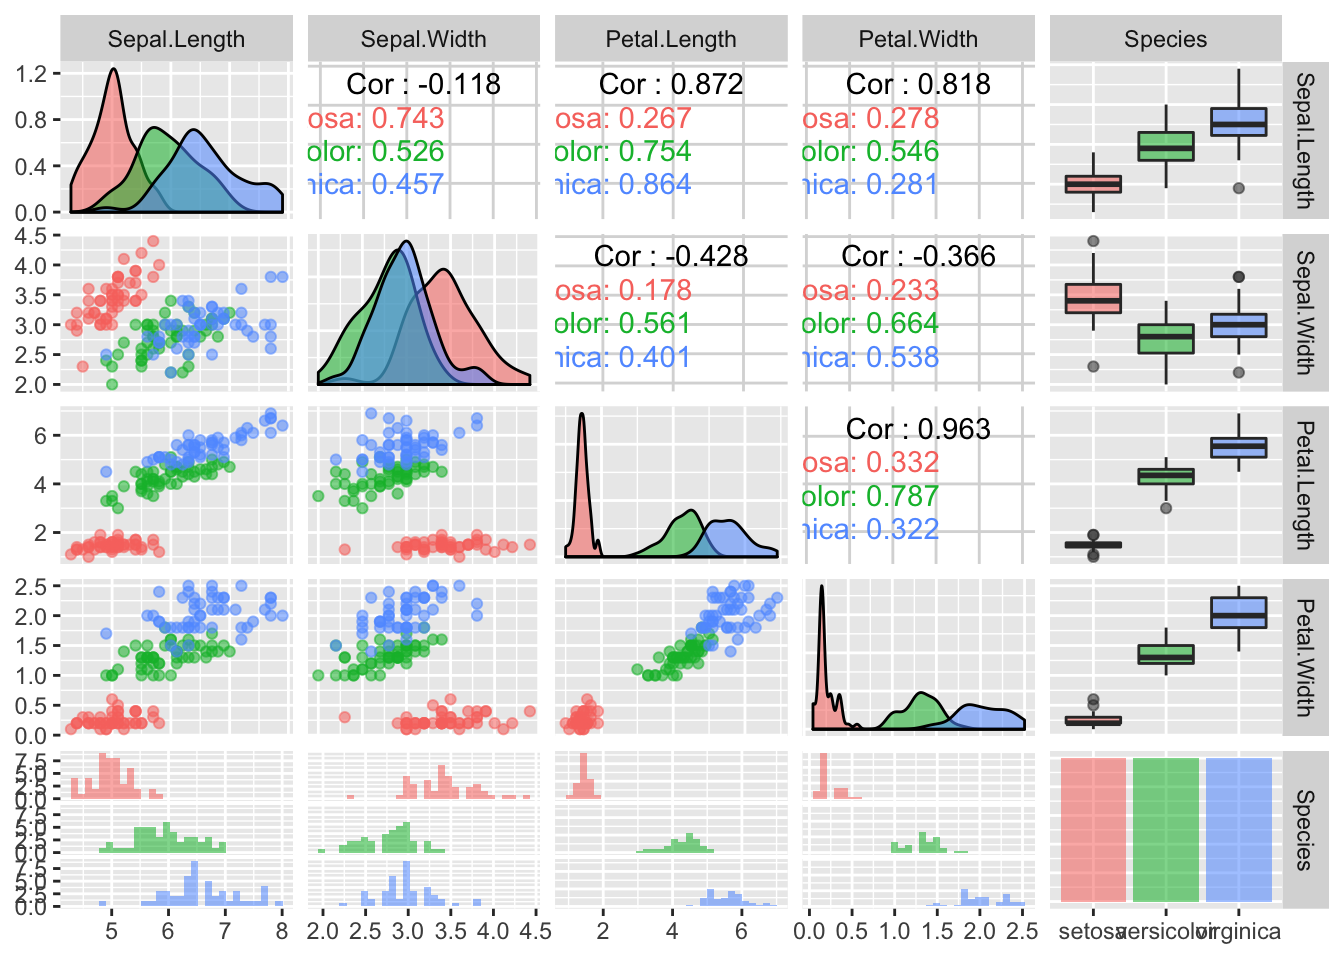
\includegraphics{R_notes_files/figure-latex/unnamed-chunk-22-1.pdf}

\section{Adding lines}\label{adding-lines}

\texttt{geom\_line()} allows you to add a simple line that joins all the
points:

\begin{Shaded}
\begin{Highlighting}[]
\KeywordTok{ggplot}\NormalTok{(iris[}\DecValTok{1}\OperatorTok{:}\DecValTok{3}\NormalTok{,], }\KeywordTok{aes}\NormalTok{(}\DataTypeTok{y =}\NormalTok{ Petal.Length, }\DataTypeTok{x =}\NormalTok{ Sepal.Length)) }\OperatorTok{+}\StringTok{ }
\StringTok{  }\KeywordTok{geom_point}\NormalTok{() }\OperatorTok{+}\StringTok{ }
\StringTok{  }\KeywordTok{geom_line}\NormalTok{()}
\end{Highlighting}
\end{Shaded}

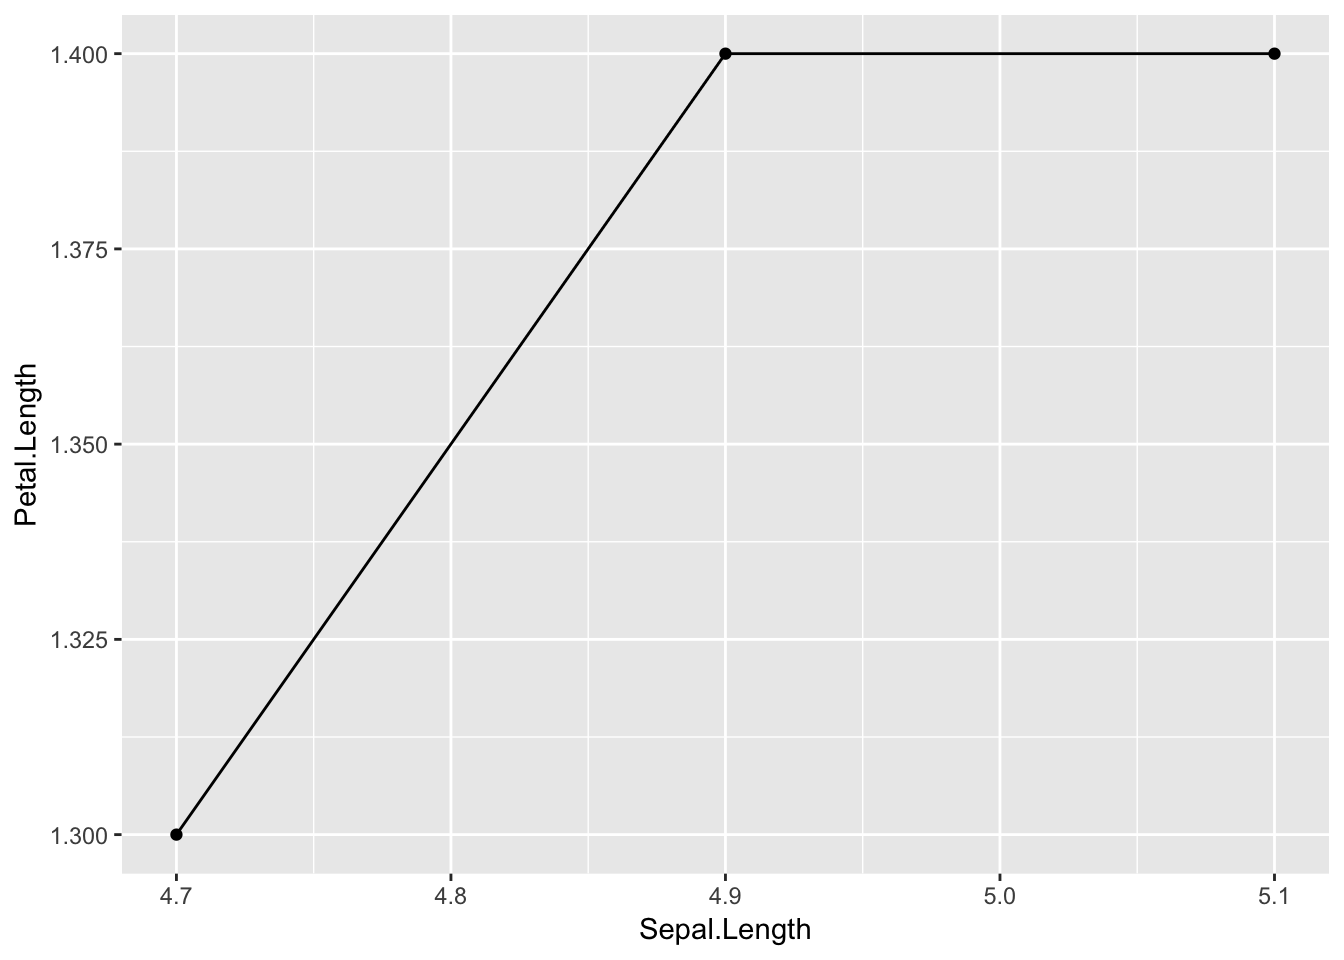
\includegraphics{R_notes_files/figure-latex/unnamed-chunk-23-1.pdf}

To change the appearance of the line, \texttt{geom\_line()} offers the
following arguments:

\begin{itemize}
\tightlist
\item
  colour
\item
  linetype
\item
  size
\end{itemize}

Setting \texttt{linetype} within \texttt{geom\_line(aes())} allows you
have different line types depending on the factor. See
\href{http://www.cookbook-r.com/Graphs/Bar_and_line_graphs_(ggplot2)/}{R
cookbook} for more details.

\texttt{geom\_smooth} allows you to fit a smooth line through all the
points using various methods. The default is `auto' which picks one of:

\begin{itemize}
\tightlist
\item
  lm
\item
  glm
\item
  gam
\item
  loess
\end{itemize}

depending on the size of the largest group. A message will be output
along with the plot informing the user of which method was used.

\begin{Shaded}
\begin{Highlighting}[]
\KeywordTok{ggplot}\NormalTok{(iris, }\KeywordTok{aes}\NormalTok{(}\DataTypeTok{y =}\NormalTok{ Petal.Width, }\DataTypeTok{x =}\NormalTok{ Petal.Length)) }\OperatorTok{+}\StringTok{ }
\StringTok{  }\KeywordTok{geom_point}\NormalTok{() }\OperatorTok{+}\StringTok{ }
\StringTok{  }\KeywordTok{geom_smooth}\NormalTok{()}
\end{Highlighting}
\end{Shaded}

\begin{verbatim}
## `geom_smooth()` using method = 'loess' and formula 'y ~ x'
\end{verbatim}

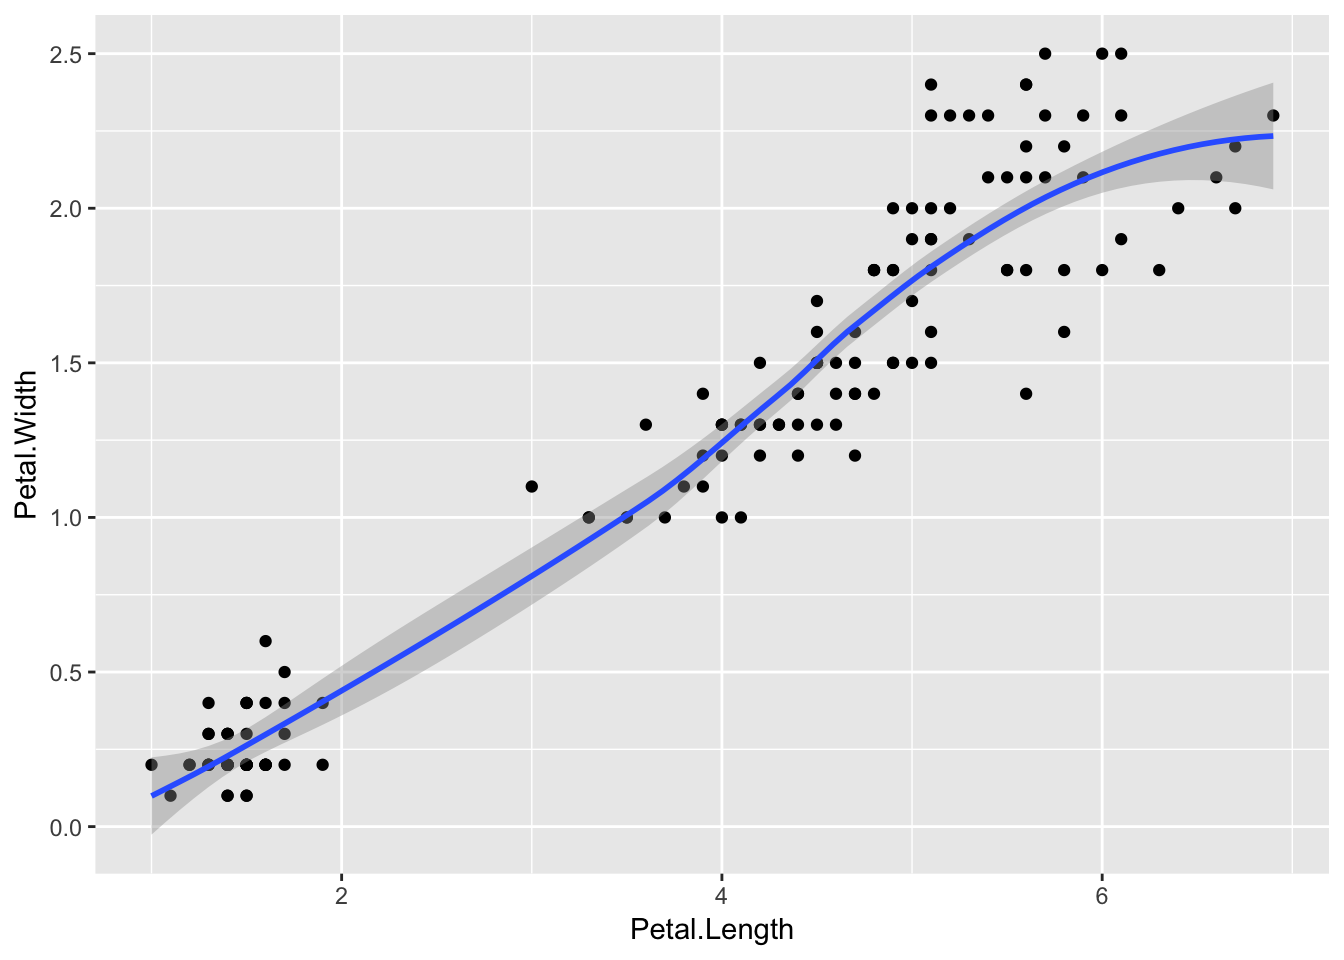
\includegraphics{R_notes_files/figure-latex/unnamed-chunk-24-1.pdf}

More details can be found in the
\href{https://ggplot2.tidyverse.org/reference/geom_smooth.html}{ggplot2
reference}.

\section{Bar graphs \& histograms}\label{bar-graphs-histograms}

The default stat of \texttt{geom\_bar()} is `count', which `bins' your
data (puts each value into a defined `bin'), and then plots bin counts.

\begin{Shaded}
\begin{Highlighting}[]
\KeywordTok{ggplot}\NormalTok{(iris, }\KeywordTok{aes}\NormalTok{(}\DataTypeTok{x =}\NormalTok{ Species)) }\OperatorTok{+}
\StringTok{  }\KeywordTok{geom_bar}\NormalTok{()}
\end{Highlighting}
\end{Shaded}

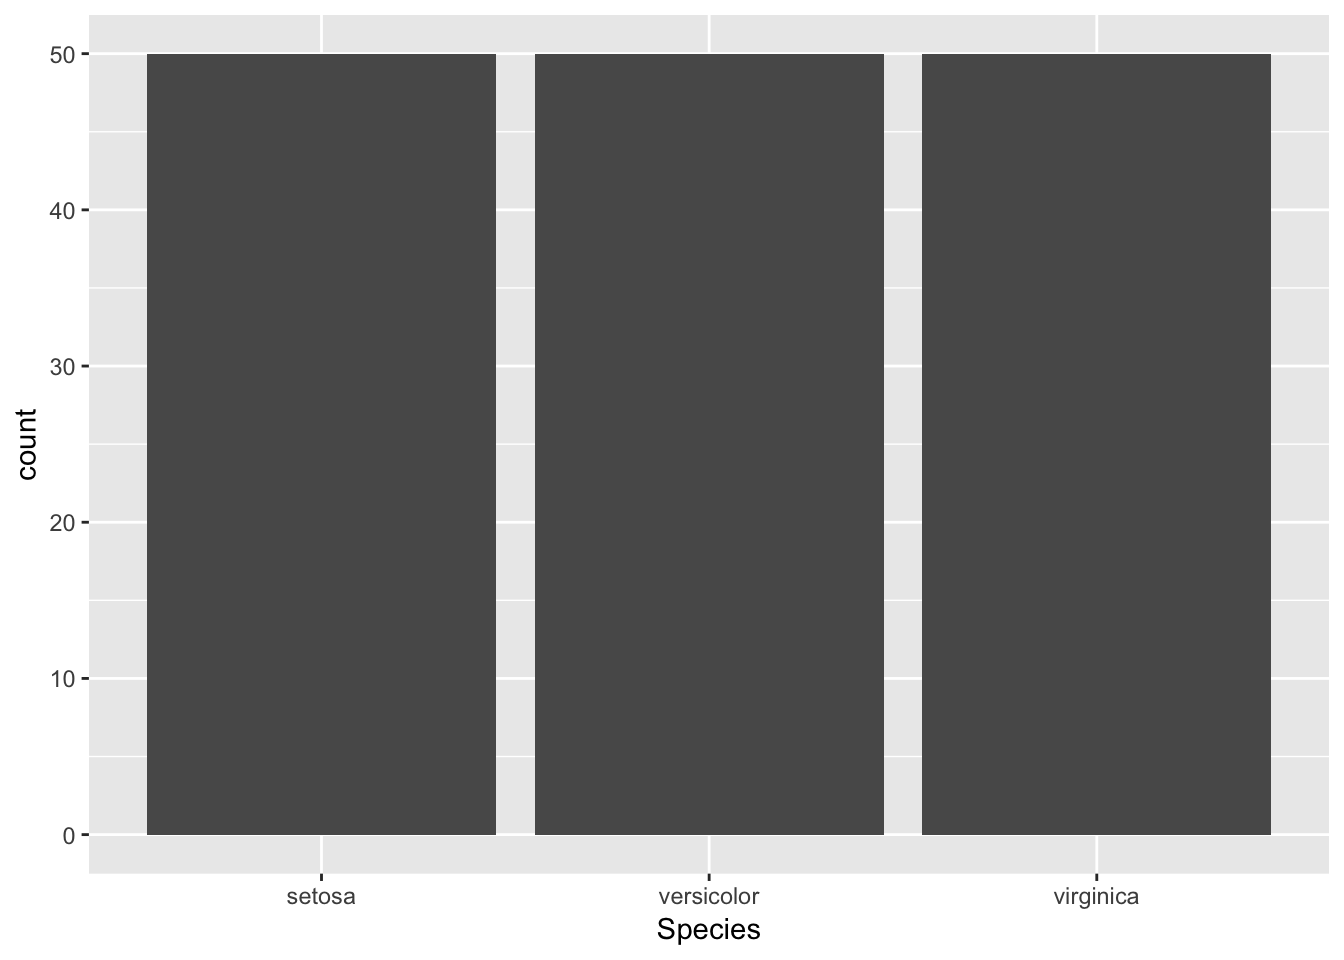
\includegraphics{R_notes_files/figure-latex/unnamed-chunk-25-1.pdf}

This tells you that there are 50 values (observations/rows) in each
species group.

\texttt{geom\_histogram()} is appropriate for a continuous variable:

\begin{Shaded}
\begin{Highlighting}[]
\KeywordTok{ggplot}\NormalTok{(iris, }\KeywordTok{aes}\NormalTok{(}\DataTypeTok{x =}\NormalTok{ Petal.Length)) }\OperatorTok{+}\StringTok{ }
\StringTok{  }\KeywordTok{geom_histogram}\NormalTok{()}
\end{Highlighting}
\end{Shaded}

\begin{verbatim}
## `stat_bin()` using `bins = 30`. Pick better value with `binwidth`.
\end{verbatim}

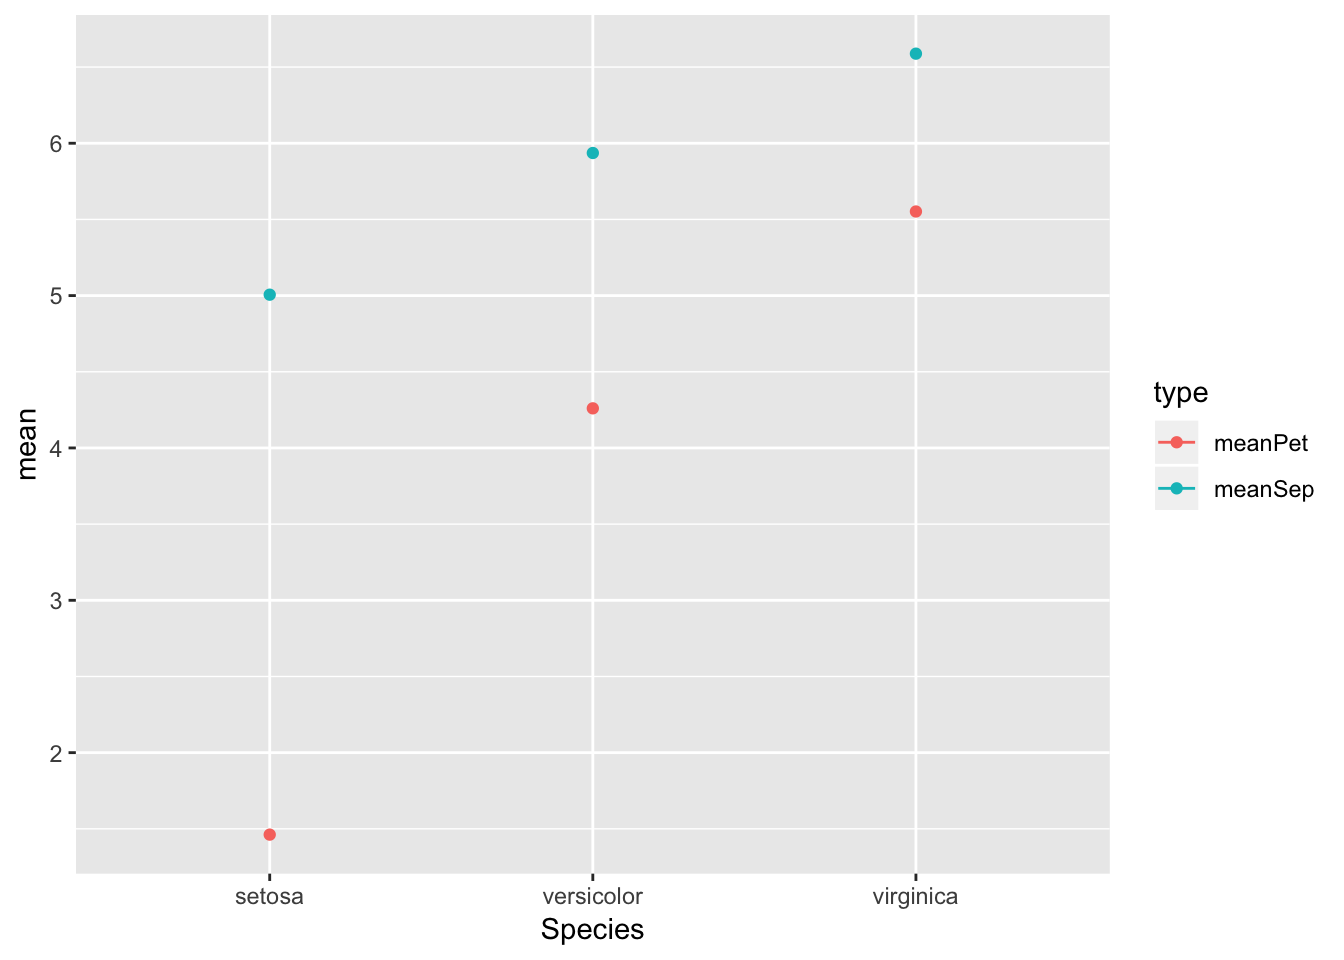
\includegraphics{R_notes_files/figure-latex/unnamed-chunk-26-1.pdf}

A message will be output with the plot telling the user which bin width
has been used. To pick a binwidth, use the \texttt{binwidth} argument in
\texttt{geom\_histogram()} (outside of \texttt{aes()}).

A number of histograms can be overlayed on top of each other, though
Hadley recommends that you do this with \texttt{geom\_freqpoly()}:

\begin{Shaded}
\begin{Highlighting}[]
\KeywordTok{ggplot}\NormalTok{(iris, }\KeywordTok{aes}\NormalTok{(}\DataTypeTok{x =}\NormalTok{ Sepal.Width, }\DataTypeTok{colour =}\NormalTok{ Species)) }\OperatorTok{+}\StringTok{ }
\StringTok{  }\KeywordTok{geom_freqpoly}\NormalTok{()}
\end{Highlighting}
\end{Shaded}

\begin{verbatim}
## `stat_bin()` using `bins = 30`. Pick better value with `binwidth`.
\end{verbatim}

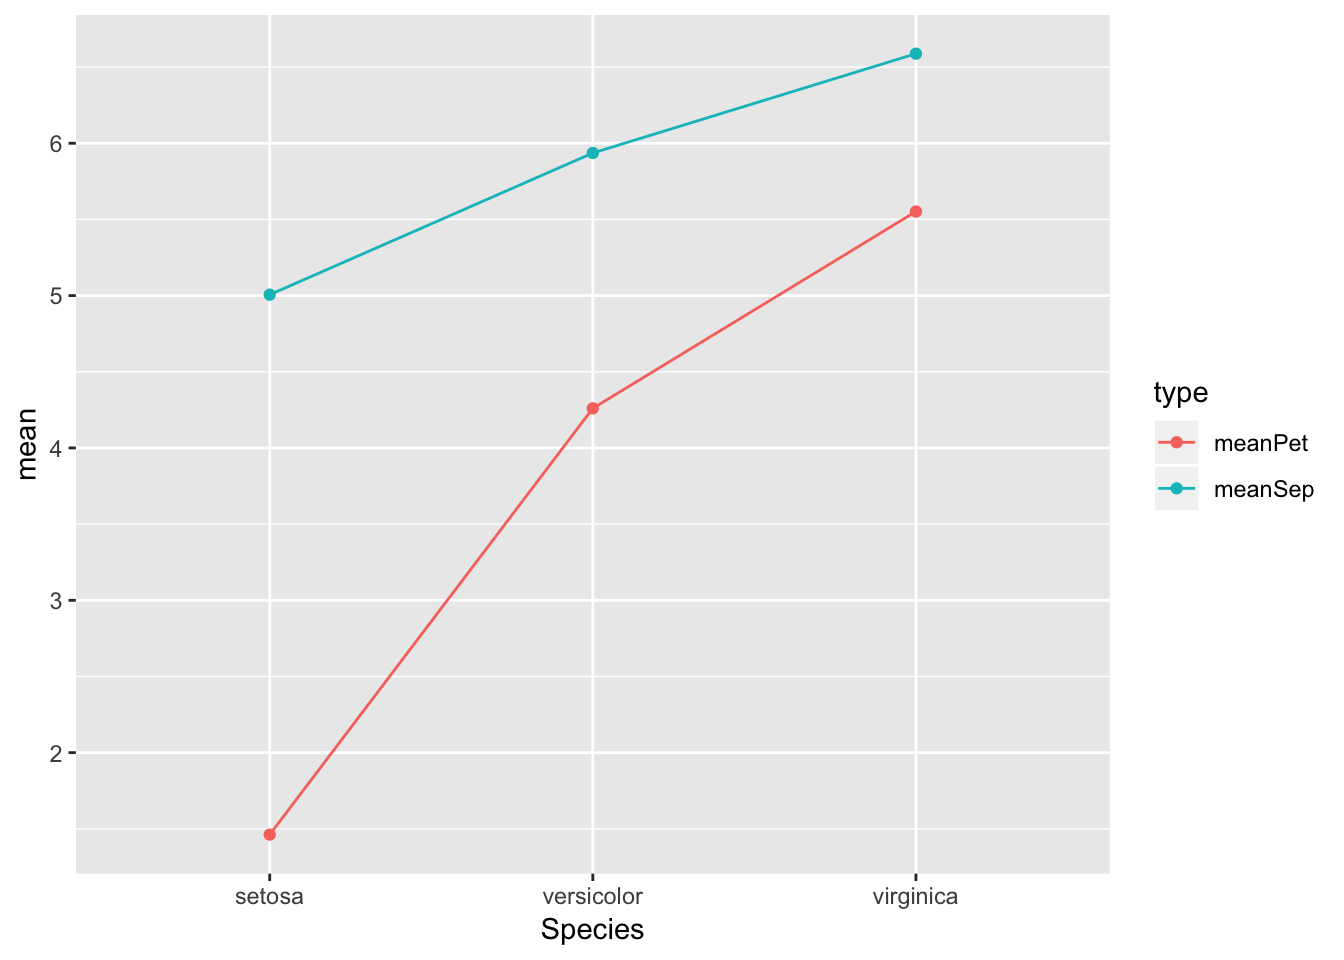
\includegraphics{R_notes_files/figure-latex/unnamed-chunk-27-1.pdf}

To plot a bar graph using absolute values (instead of frequencies), use
\texttt{stat\ =\ \textquotesingle{}identity\textquotesingle{}} (see 888
chapter for dplyr notation):

\begin{Shaded}
\begin{Highlighting}[]
\NormalTok{iris }\OperatorTok
\StringTok{  }\KeywordTok{group_by}\NormalTok{(Species) }\OperatorTok
\StringTok{  }\KeywordTok{summarise}\NormalTok{(}\DataTypeTok{mean =} \KeywordTok{mean}\NormalTok{(Sepal.Length)) }\OperatorTok
\StringTok{  }\KeywordTok{ggplot}\NormalTok{(}\KeywordTok{aes}\NormalTok{(}\DataTypeTok{y =}\NormalTok{ mean, }\DataTypeTok{x =}\NormalTok{ Species)) }\OperatorTok{+}\StringTok{ }
\StringTok{  }\KeywordTok{geom_bar}\NormalTok{(}\DataTypeTok{stat =} \StringTok{'identity'}\NormalTok{)}
\end{Highlighting}
\end{Shaded}

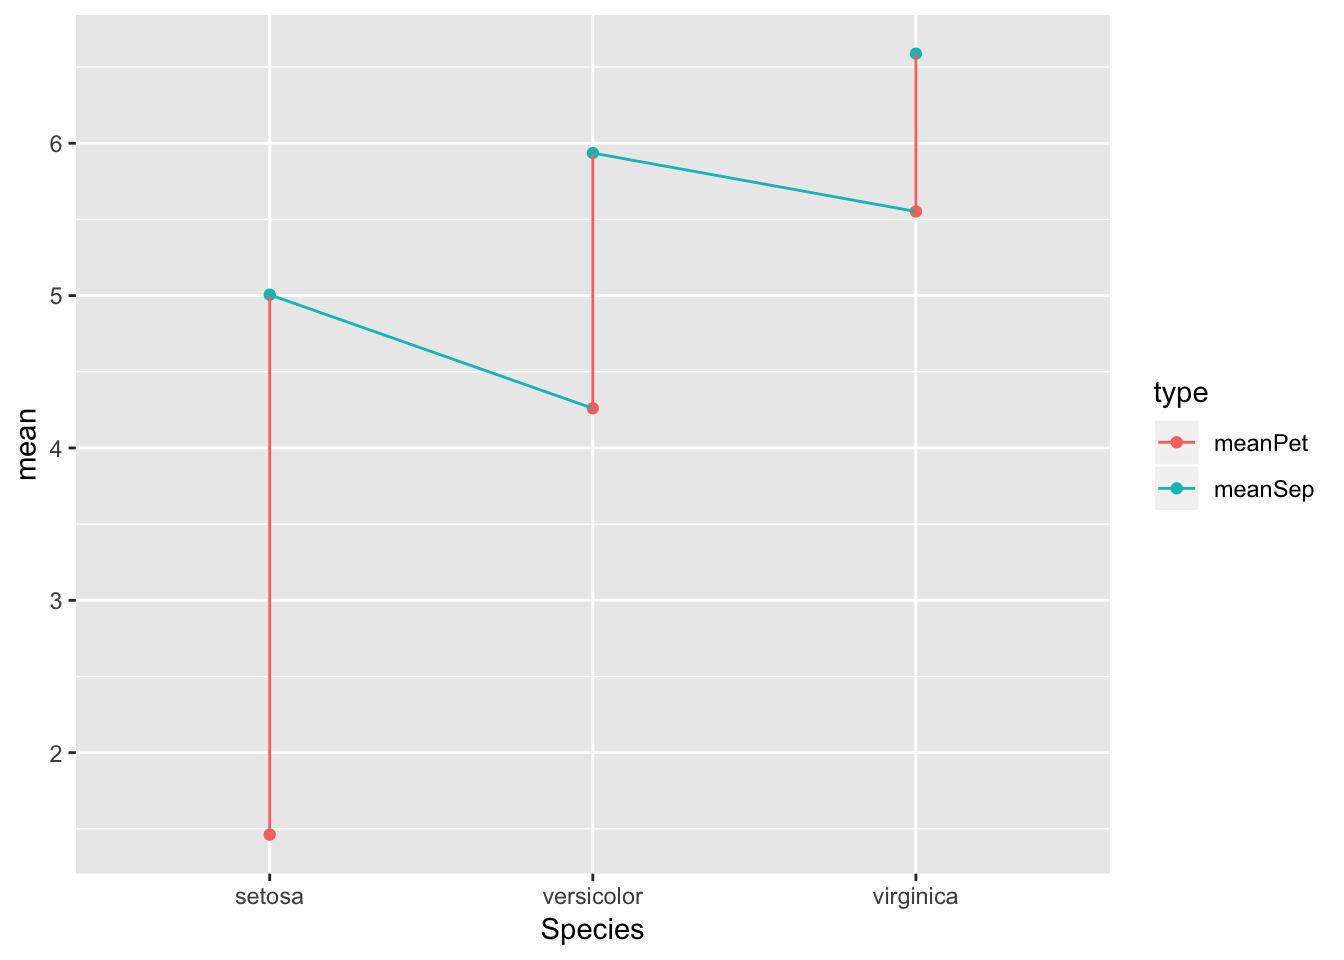
\includegraphics{R_notes_files/figure-latex/unnamed-chunk-28-1.pdf}

Adding \texttt{fill} argument in \texttt{aes()} will create a stacked
bar graph:

\begin{Shaded}
\begin{Highlighting}[]
\KeywordTok{ggplot}\NormalTok{(iris, }\KeywordTok{aes}\NormalTok{(}\DataTypeTok{x =}\NormalTok{ Sepal.Length, }\DataTypeTok{fill =}\NormalTok{ Species)) }\OperatorTok{+}\StringTok{ }
\StringTok{  }\KeywordTok{geom_bar}\NormalTok{()}
\end{Highlighting}
\end{Shaded}

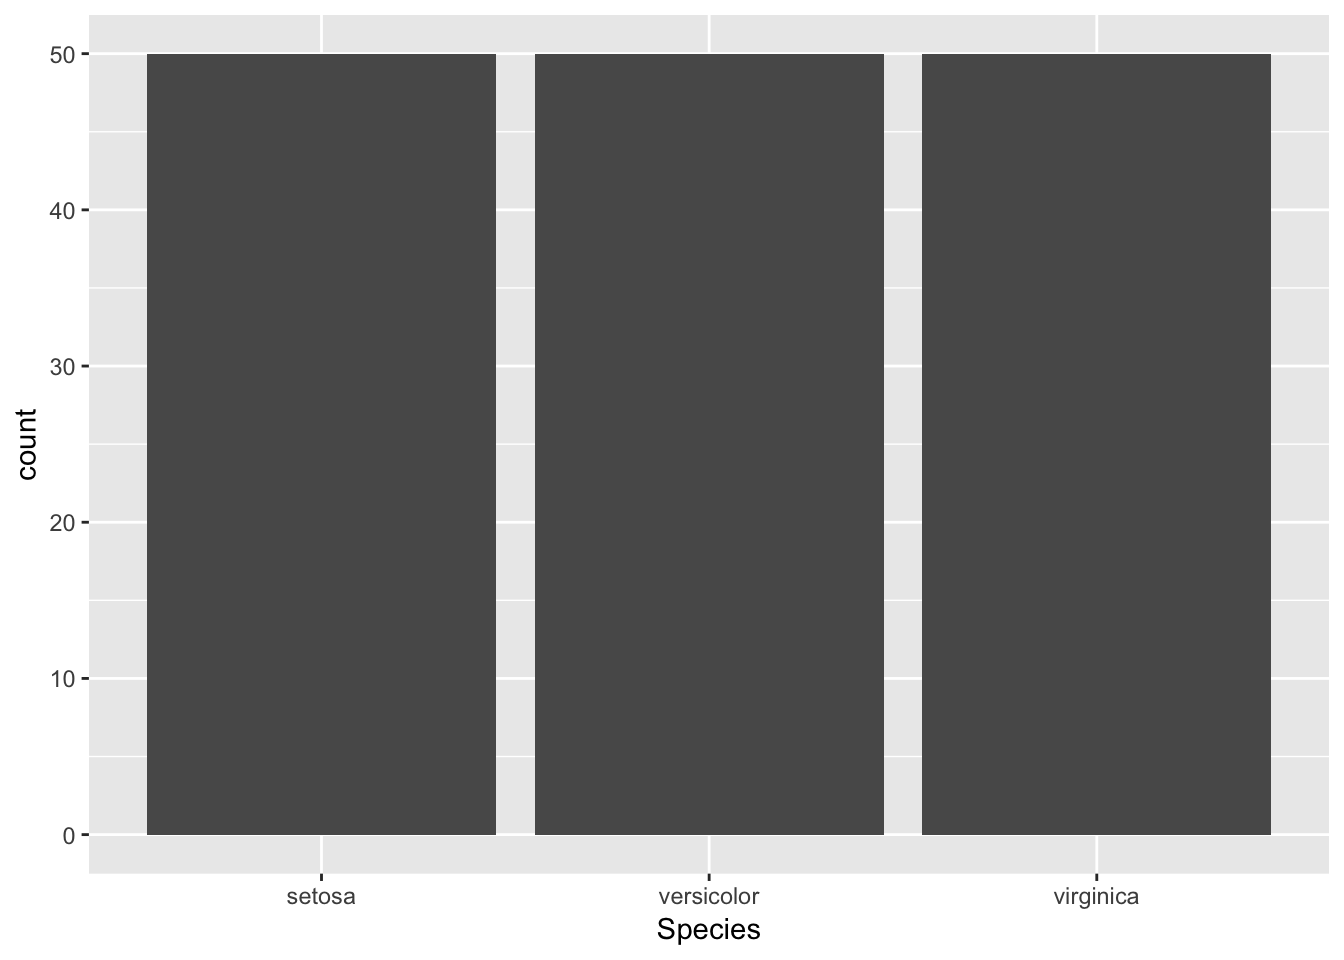
\includegraphics{R_notes_files/figure-latex/unnamed-chunk-29-1.pdf}

Note: \texttt{fill} species the colour of the bar (or point) and
\texttt{colour} spefies the colour of the border around the bar (or
point).

To have the bars next to each other instead of stacked, use
\texttt{position\ =\ \textquotesingle{}dodge\textquotesingle{}}:

\begin{Shaded}
\begin{Highlighting}[]
\KeywordTok{ggplot}\NormalTok{(iris, }\KeywordTok{aes}\NormalTok{(}\DataTypeTok{x =}\NormalTok{ Sepal.Length, }\DataTypeTok{fill =}\NormalTok{ Species)) }\OperatorTok{+}\StringTok{ }
\StringTok{  }\KeywordTok{geom_bar}\NormalTok{(}\DataTypeTok{position =} \StringTok{'dodge'}\NormalTok{)}
\end{Highlighting}
\end{Shaded}

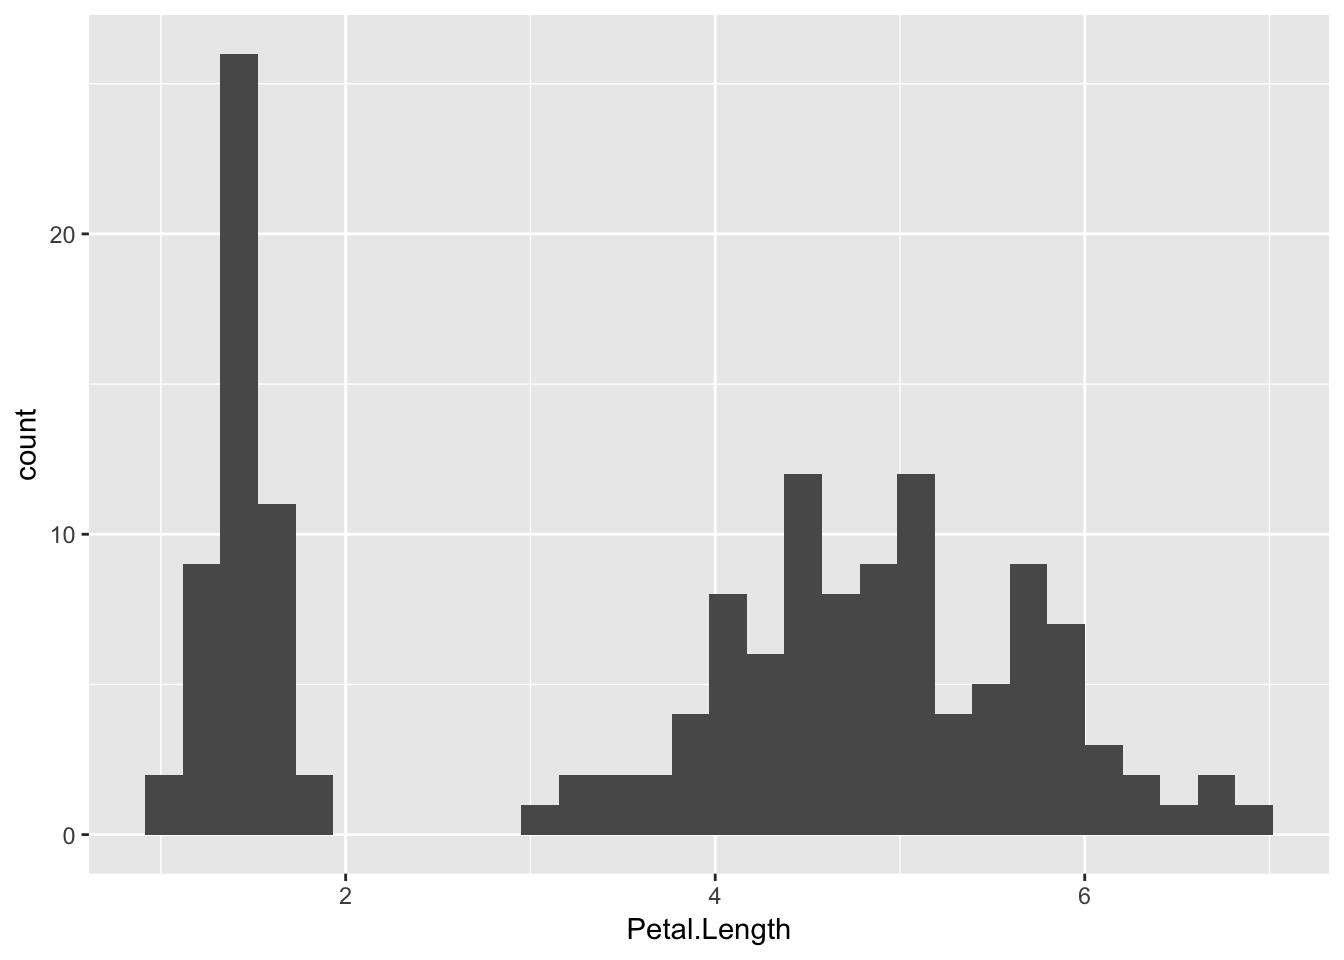
\includegraphics{R_notes_files/figure-latex/unnamed-chunk-30-1.pdf}

Note in the graph above, for lengths where not all species are present,
there is only 1 bar that is wider. To fix this - google it\ldots{}

\section{geom\_boxplot}\label{geom_boxplot}

Definitions: * A box that stretches from the 25th percentile of the
distribution to the 75th percentile * A line (or whisker) that extends
from each end of the box and goes to the farthest non-outlier point in
the distribution. * Points (dots) that display observations that fall
more than 1.5 times the IQR from either edge of the box. These outlying
points are unusual so are plotted individually.

\section{Facets}\label{facets}

(Back to the \texttt{mpg} dataset)

Another way to add variables is to split into many graphs:

\begin{Shaded}
\begin{Highlighting}[]
\KeywordTok{ggplot}\NormalTok{(mpg) }\OperatorTok{+}\StringTok{ }
\StringTok{  }\KeywordTok{geom_point}\NormalTok{(}\KeywordTok{aes}\NormalTok{(}\DataTypeTok{x =}\NormalTok{ displ, }\DataTypeTok{y =}\NormalTok{ hwy)) }\OperatorTok{+}\StringTok{ }
\StringTok{  }\KeywordTok{facet_wrap}\NormalTok{(. }\OperatorTok{~}\StringTok{ }\NormalTok{class, }\DataTypeTok{nrow =} \DecValTok{2}\NormalTok{) }\CommentTok{# same plot with or without dot}
\end{Highlighting}
\end{Shaded}

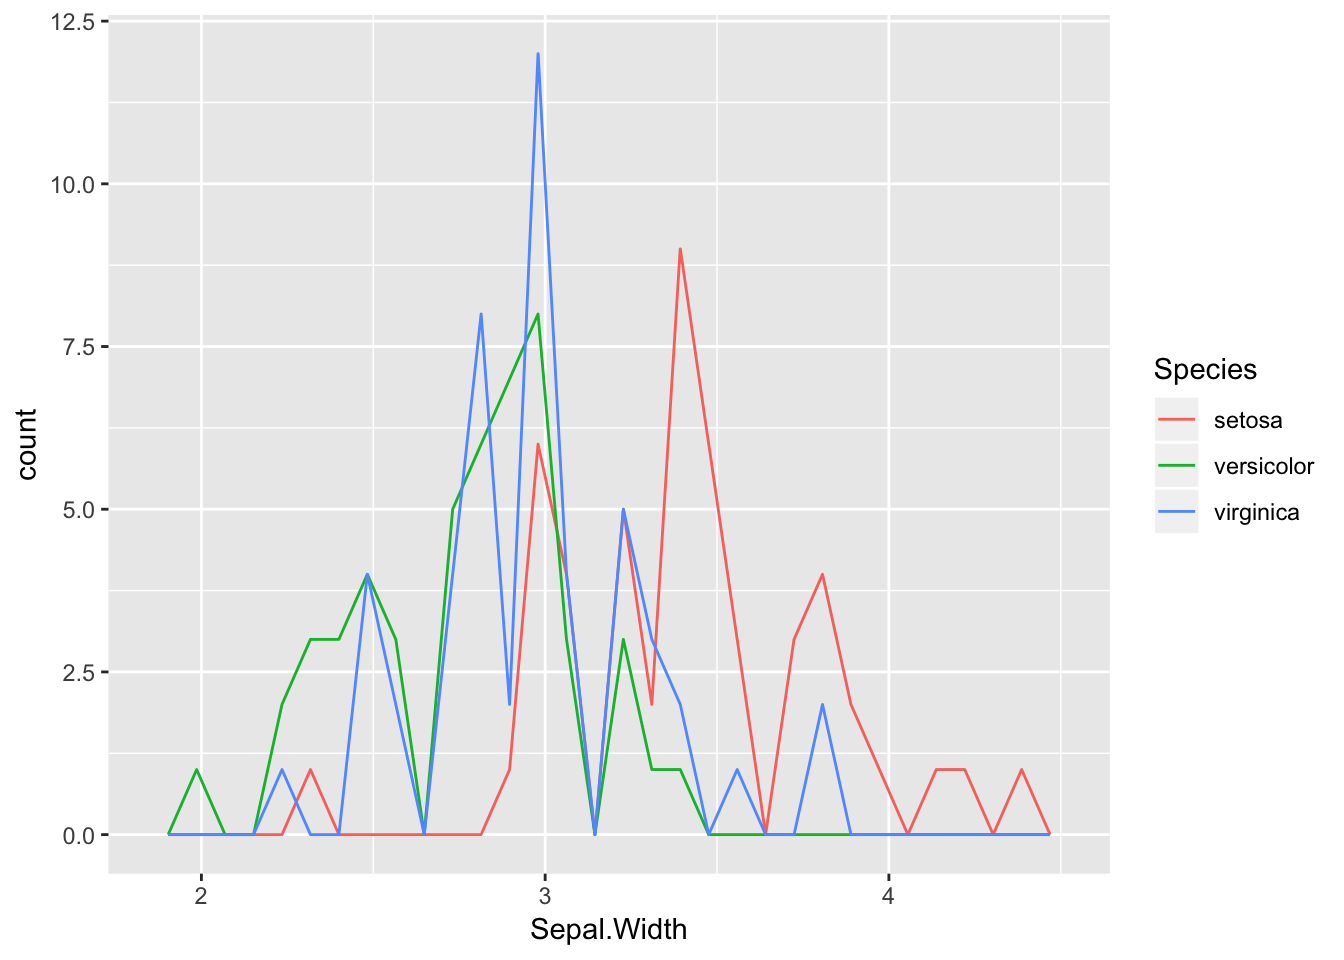
\includegraphics{R_notes_files/figure-latex/unnamed-chunk-31-1.pdf}

The first argument is a `formula', which you create with
\texttt{\textasciitilde{}} followed by variable name. Variable should
not be a continuous variable. In the above plot, leaving one side empty
or using a dot means that only one variable is being facetted. The
\texttt{nrow} and \texttt{ncol} arguments let you specify how many rows
or columns you want.

If you wish to facet using two variables, \texttt{facet\_wrap} will look
like this:

\begin{Shaded}
\begin{Highlighting}[]
\KeywordTok{ggplot}\NormalTok{(mpg) }\OperatorTok{+}\StringTok{ }
\StringTok{  }\KeywordTok{geom_point}\NormalTok{(}\KeywordTok{aes}\NormalTok{(}\DataTypeTok{x =}\NormalTok{ displ, }\DataTypeTok{y =}\NormalTok{ hwy)) }\OperatorTok{+}\StringTok{ }
\StringTok{  }\KeywordTok{facet_wrap}\NormalTok{(drv }\OperatorTok{~}\StringTok{ }\NormalTok{class, }\DataTypeTok{nrow =} \DecValTok{2}\NormalTok{) }\CommentTok{# same plot with or without dot}
\end{Highlighting}
\end{Shaded}

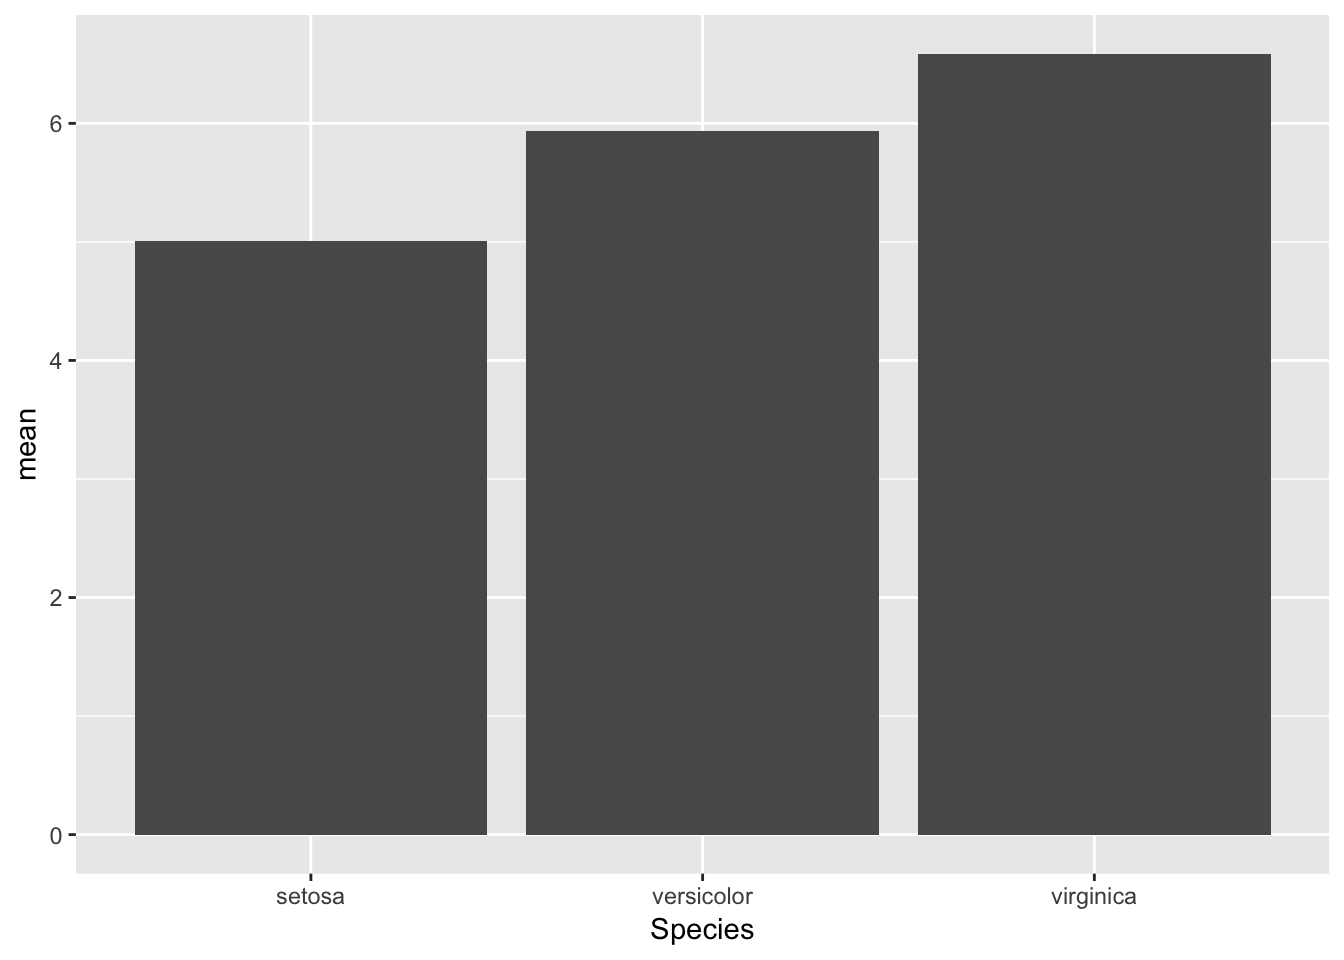
\includegraphics{R_notes_files/figure-latex/unnamed-chunk-32-1.pdf}

Graphs for all possible combinations of your two variables are created
and arranged as per the \texttt{nrow} and \texttt{ncol} specification -
as described by the help file: `Wrap a 1d ribbon of panels into 2d'.
Note that only combinations where there values are shown.

Alternatively you can use \texttt{facet\_grid()}:

\begin{Shaded}
\begin{Highlighting}[]
\KeywordTok{ggplot}\NormalTok{(mpg) }\OperatorTok{+}\StringTok{ }
\StringTok{  }\KeywordTok{geom_point}\NormalTok{(}\KeywordTok{aes}\NormalTok{(}\DataTypeTok{x =}\NormalTok{ displ, }\DataTypeTok{y =}\NormalTok{ hwy)) }\OperatorTok{+}\StringTok{ }
\StringTok{  }\KeywordTok{facet_grid}\NormalTok{(drv }\OperatorTok{~}\StringTok{ }\NormalTok{cyl)}
\end{Highlighting}
\end{Shaded}

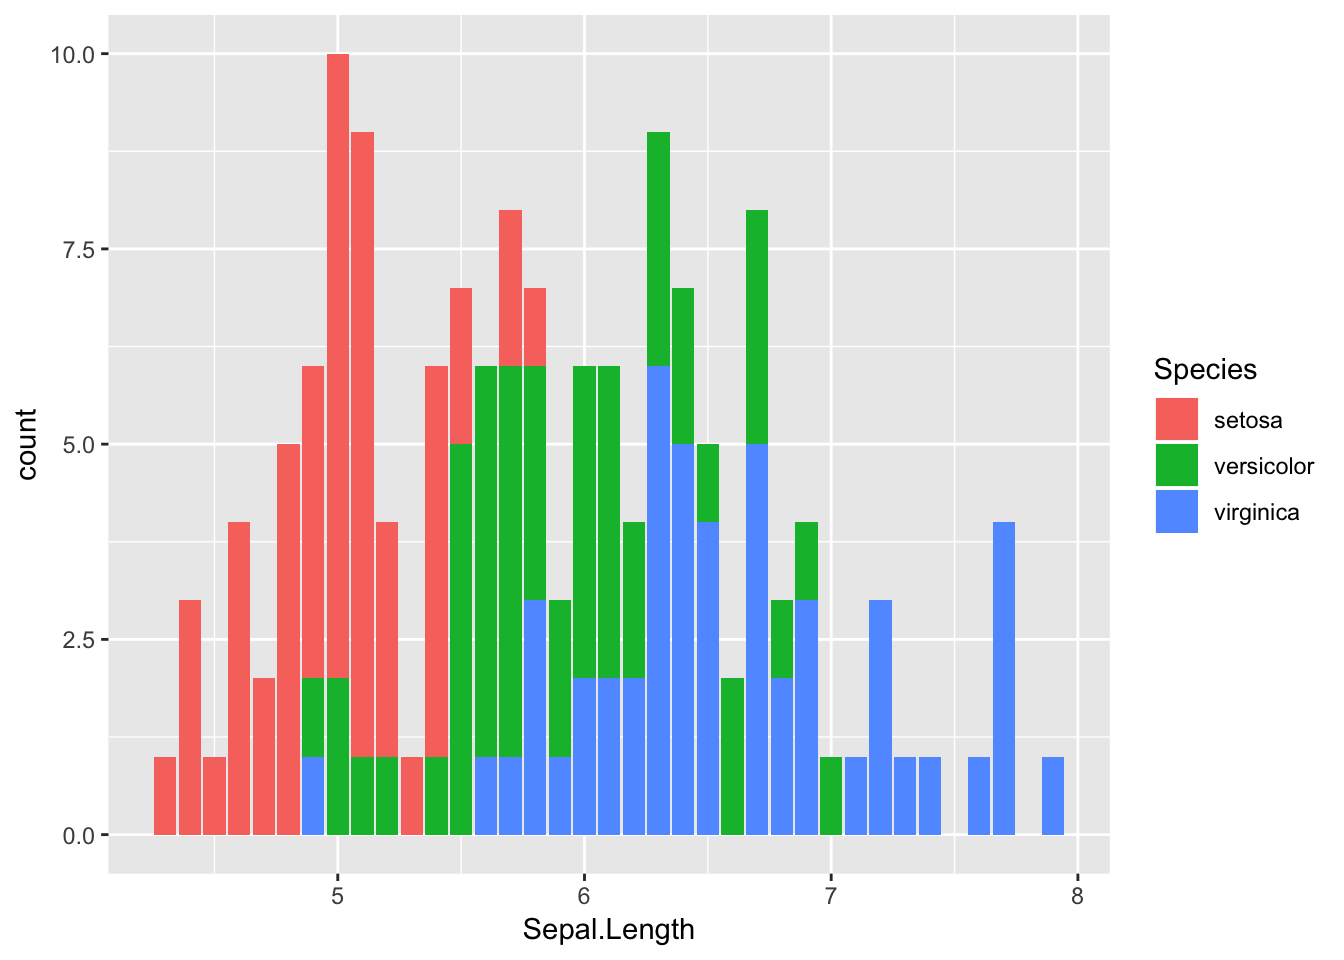
\includegraphics{R_notes_files/figure-latex/unnamed-chunk-33-1.pdf}

Here the notation is \texttt{(row\ \textasciitilde{}\ column)} - LHS is
which variable should be horizontally facetted and RHS is which variable
should be vertically facetted.

Note that in this case graphs for all possible combinations of the two
variables are created, even though some combinations have no values
(e.g.~the botton left graphs have no points in them).

\section{Reordering factors}\label{reordering-factors}

Often a specific order of factor levels is desired when plotting. This
can be achieved using the base R function \texttt{reorder()}.

\begin{Shaded}
\begin{Highlighting}[]
\KeywordTok{head}\NormalTok{(}
\KeywordTok{reorder}\NormalTok{(mpg}\OperatorTok{$}\NormalTok{manufacturer, mpg}\OperatorTok{$}\NormalTok{displ, }\DataTypeTok{FUN =}\NormalTok{ max),}
\DataTypeTok{n=}\DecValTok{20}
\NormalTok{)}
\end{Highlighting}
\end{Shaded}

\begin{verbatim}
##  [1] audi      audi      audi      audi      audi      audi      audi     
##  [8] audi      audi      audi      audi      audi      audi      audi     
## [15] audi      audi      audi      audi      chevrolet chevrolet
## 15 Levels: honda subaru hyundai volkswagen audi land rover ... chevrolet
\end{verbatim}

In the above code we have reordered the levels of
\texttt{mpg\$manufacturer} according to the maximum \texttt{mpg\$displ}
(engine displacement in litres) value of each factor group. See the
\texttt{reorder} help file for more details.

\begin{Shaded}
\begin{Highlighting}[]
\KeywordTok{ggplot}\NormalTok{(mpg) }\OperatorTok{+}
\StringTok{  }\KeywordTok{geom_boxplot}\NormalTok{(}\KeywordTok{aes}\NormalTok{(}\DataTypeTok{x =} \KeywordTok{reorder}\NormalTok{(class, hwy, }\DataTypeTok{FUN =}\NormalTok{ median), }\DataTypeTok{y =}\NormalTok{ hwy))}
\end{Highlighting}
\end{Shaded}

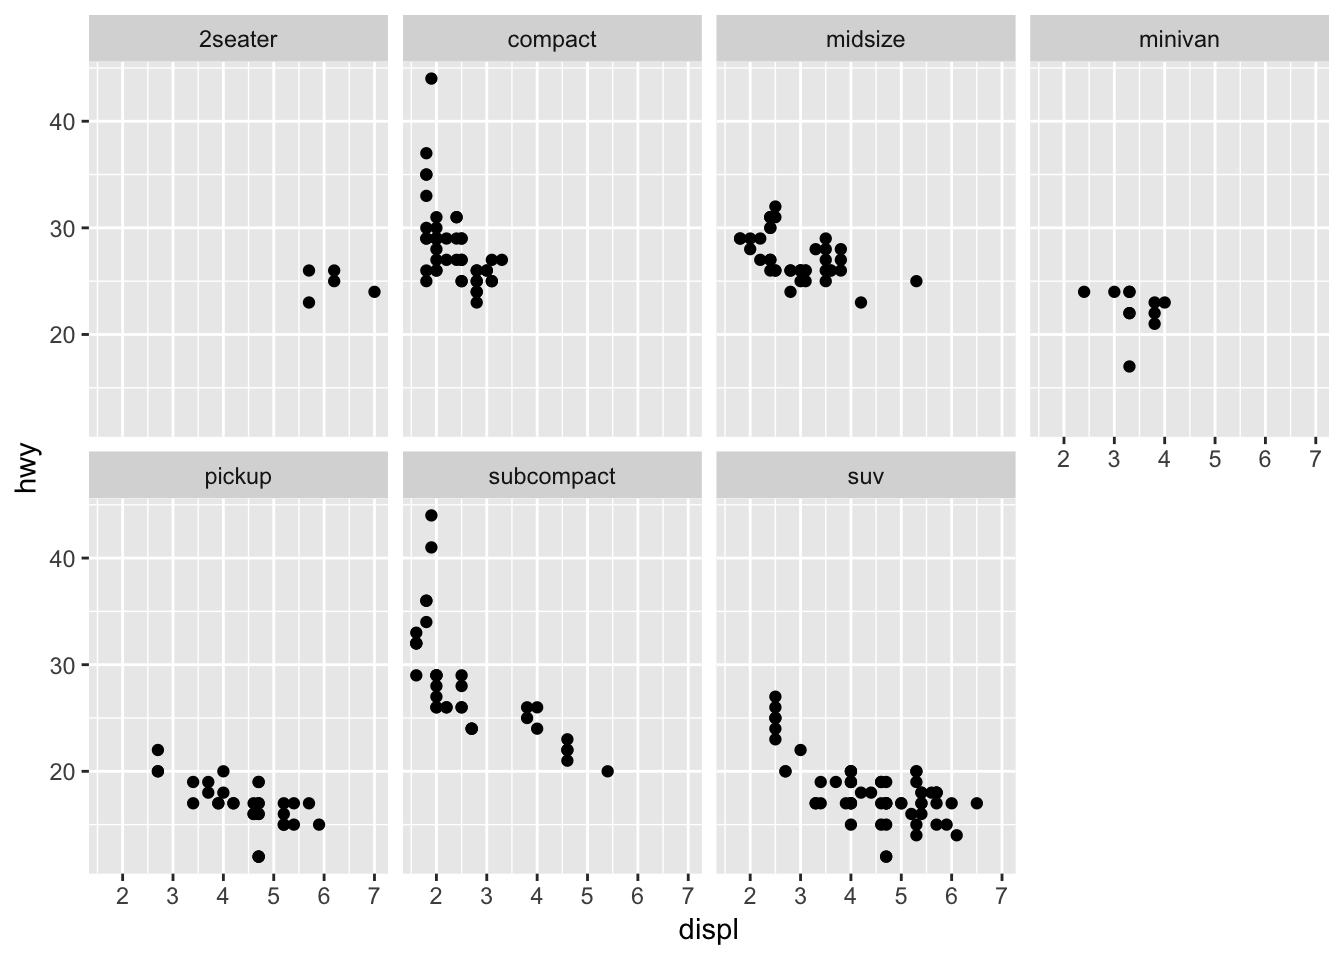
\includegraphics{R_notes_files/figure-latex/unnamed-chunk-35-1.pdf}

In the above graph, we have reordered the levels of \texttt{mpg\$class}
according to their median hwy levels. You acn see in the boxplot, that
the median hwy levels increase from left to right.

\section{Coordinate systems}\label{coordinate-systems}

Default is Cartesian.

\texttt{coord\_flip()} switches axis of the graph - rotatwa graph by 90
deg. Good for graphs with long names on the x-axis.
\texttt{coord\_cartesian(ylim\ =\ c(min,max),\ xlim\ =\ c(min,max))}
lets you `zoom' in on a particular part of the graph.

\section{Reference lines}\label{reference-lines}

Reference lines can be added to graphs using:

\begin{itemize}
\tightlist
\item
  \texttt{geom\_abline} - diagonal specified by slope and intercept
  (vertical and horizontal lines can also be drawn)
\item
  \texttt{geom\_hline} - horizontal line
\item
  \texttt{geom\_vline} - vertical line
\end{itemize}

See
\href{https://ggplot2.tidyverse.org/reference/geom_abline.html}{ggplot
reference} for examples.

\section{Error bars}\label{error-bars}

To add error bars, you must specify the length of each error bar. For
example, if you wished to have +/- standard deviation error bars on a
bar graph, you need to have a column in your dataframe with the standard
deviation for each bar.

If we wanted to plot the mean +/- sd of the Sepal.Length we would need a
dataframe with these columns:

\begin{Shaded}
\begin{Highlighting}[]
\NormalTok{iris }\OperatorTok
\StringTok{  }\KeywordTok{group_by}\NormalTok{(Species) }\OperatorTok
\StringTok{  }\KeywordTok{summarise}\NormalTok{(}\DataTypeTok{mean =} \KeywordTok{mean}\NormalTok{(Sepal.Length), }\DataTypeTok{sd =} \KeywordTok{sd}\NormalTok{(Sepal.Length)) }
\end{Highlighting}
\end{Shaded}

\begin{verbatim}
## # A tibble: 3 x 3
##   Species     mean    sd
##   <fct>      <dbl> <dbl>
## 1 setosa      5.01 0.352
## 2 versicolor  5.94 0.516
## 3 virginica   6.59 0.636
\end{verbatim}

To add the error bars, use \texttt{geom\_eerrobar()}:

\begin{Shaded}
\begin{Highlighting}[]
\NormalTok{iris }\OperatorTok
\StringTok{  }\KeywordTok{group_by}\NormalTok{(Species) }\OperatorTok
\StringTok{  }\KeywordTok{summarise}\NormalTok{(}\DataTypeTok{mean =} \KeywordTok{mean}\NormalTok{(Sepal.Length), }\DataTypeTok{sd =} \KeywordTok{sd}\NormalTok{(Sepal.Length)) }\OperatorTok
\StringTok{  }\KeywordTok{ggplot}\NormalTok{(}\KeywordTok{aes}\NormalTok{(}\DataTypeTok{y =}\NormalTok{ mean, }\DataTypeTok{x =}\NormalTok{ Species)) }\OperatorTok{+}\StringTok{ }
\StringTok{  }\KeywordTok{geom_bar}\NormalTok{(}\DataTypeTok{stat =} \StringTok{'identity'}\NormalTok{) }\OperatorTok{+}\StringTok{ }
\StringTok{  }\KeywordTok{geom_errorbar}\NormalTok{(}\KeywordTok{aes}\NormalTok{(}\DataTypeTok{ymin =}\NormalTok{ mean }\OperatorTok{-}\StringTok{ }\NormalTok{sd, }\DataTypeTok{ymax =}\NormalTok{ mean }\OperatorTok{+}\StringTok{ }\NormalTok{sd))}
\end{Highlighting}
\end{Shaded}

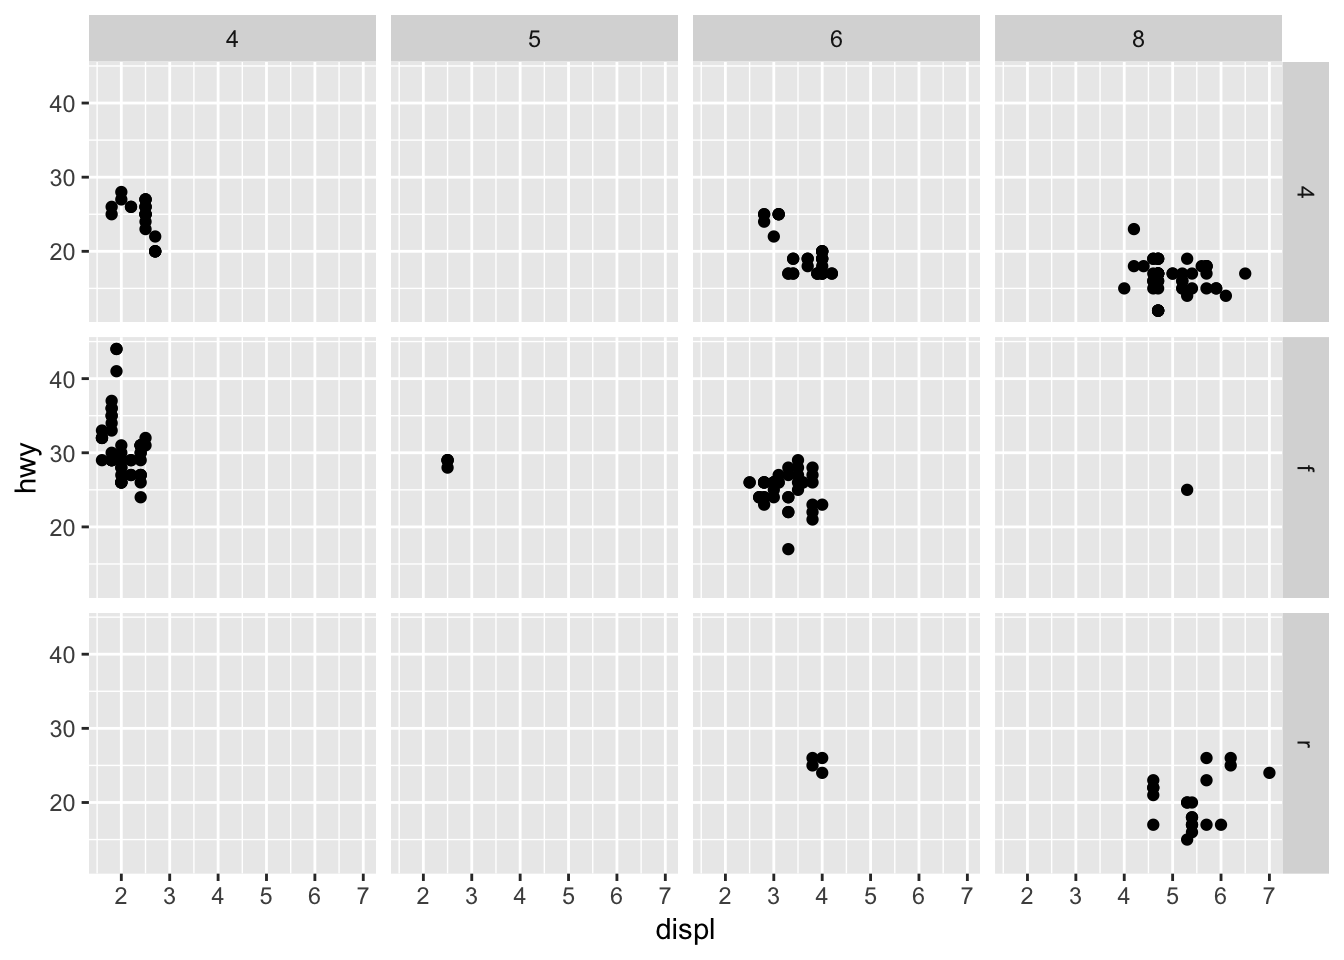
\includegraphics{R_notes_files/figure-latex/unnamed-chunk-37-1.pdf}

To change the appearance of the error bar, there are many options:

\begin{Shaded}
\begin{Highlighting}[]
\NormalTok{iris }\OperatorTok
\StringTok{  }\KeywordTok{group_by}\NormalTok{(Species) }\OperatorTok
\StringTok{  }\KeywordTok{summarise}\NormalTok{(}\DataTypeTok{mean =} \KeywordTok{mean}\NormalTok{(Sepal.Length), }\DataTypeTok{sd =} \KeywordTok{sd}\NormalTok{(Sepal.Length)) }\OperatorTok
\StringTok{  }\KeywordTok{ggplot}\NormalTok{(}\KeywordTok{aes}\NormalTok{(}\DataTypeTok{y =}\NormalTok{ mean, }\DataTypeTok{x =}\NormalTok{ Species)) }\OperatorTok{+}\StringTok{ }
\StringTok{  }\KeywordTok{geom_bar}\NormalTok{(}\DataTypeTok{stat =} \StringTok{'identity'}\NormalTok{) }\OperatorTok{+}\StringTok{ }
\StringTok{  }\KeywordTok{geom_errorbar}\NormalTok{(}\KeywordTok{aes}\NormalTok{(}\DataTypeTok{ymin =}\NormalTok{ mean }\OperatorTok{-}\StringTok{ }\NormalTok{sd, }\DataTypeTok{ymax =}\NormalTok{ mean }\OperatorTok{+}\StringTok{ }\NormalTok{sd),}
                \DataTypeTok{size =} \FloatTok{0.3}\NormalTok{, }\CommentTok{# thinner lines}
                \DataTypeTok{width =} \FloatTok{0.2}\NormalTok{, }\CommentTok{# how much of the bar the error bar should span}
                \DataTypeTok{position =} \KeywordTok{position_dodge}\NormalTok{(}\FloatTok{0.9}\NormalTok{)}
\NormalTok{                )}
\end{Highlighting}
\end{Shaded}

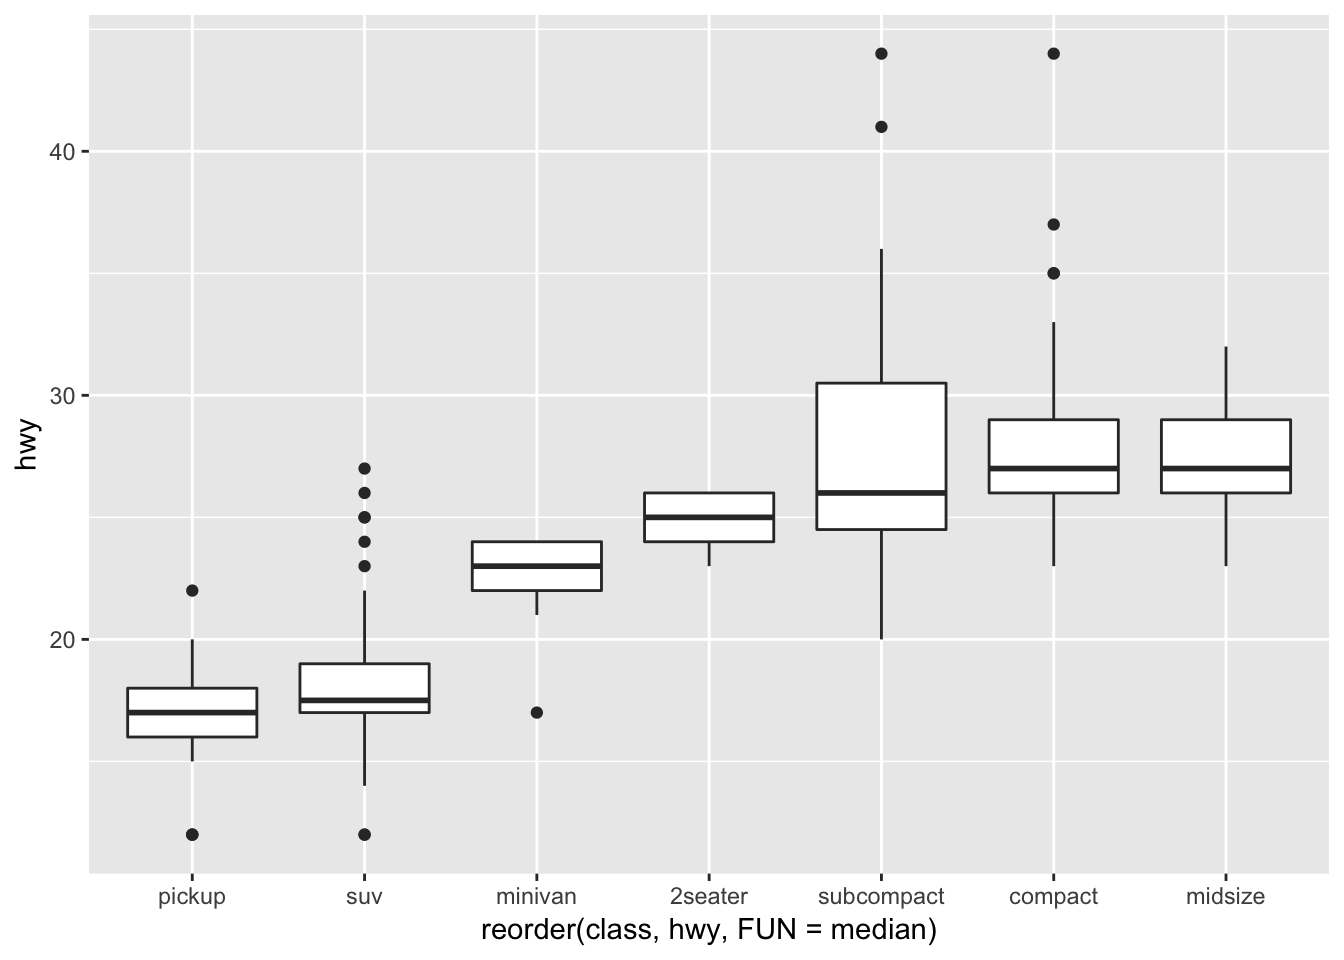
\includegraphics{R_notes_files/figure-latex/unnamed-chunk-38-1.pdf}

\texttt{position\_dodge()} preserves the vertical position of an geom
while adjusting the horizontal position. (see
\href{https://ggplot2.tidyverse.org/reference/position_dodge.html}{ggplot
ref} for more details)

For more examples see
\href{http://www.cookbook-r.com/Graphs/Plotting_means_and_error_bars_(ggplot2)/}{R
cookbook}.

\section{Appearance}\label{appearance}

\begin{itemize}
\tightlist
\item
  Change axis name and title:
  \texttt{labs(title\ =\ "MAIN\ TITLE",\ x\ =\ "X-AXIS\ TITLE",\ y\ =\ "Y-AXIS\ TITLE")}
\item
  Change position of title:
  \texttt{theme(plot.title\ =\ element\_text(hjust\ =\ 0.5))}
\item
  Set which categories appear in barplot/boxplot:
  \texttt{xlim("Category1","Category2")}
\item
  Change colour of \texttt{fill} boxplot/bars:
  \texttt{scale\_fill\_manual(values\ =\ c("Colour1",\ "Colour2"),\ name\ =\ "title\ of\ Legend",\ labels\ =\ c("Label1","Label2"))}
\item
  Change names under each bar/boxplot:
  \texttt{Change\ names\ under\ each\ bar/boxplot}
\item
  Change title text style:
  \texttt{theme(title\ =\ element\_text(face\ =\ "bold.italic",\ color\ =\ "blue",\ size\ =\ 16))}
\item
  Change axis name text style:
  \texttt{theme(axis.title\ =\ element\_text(face\ =\ "bold.italic",\ color\ =\ "red",\ size\ =\ 16))}
\item
  Legend title/labels:
  \texttt{scale\_fill\_discrete(name\ =\ "Legend\ name",\ labels\ =\ c())}
\item
  Angle of labels:
  \texttt{theme(axis.text.x\ =\ element\_text(angle\ =\ 90,\ hjust\ =\ 1))}
\end{itemize}

Fonts: \href{http://www.cookbook-r.com/Graphs/Fonts/}{cookbook}

\section{dplyr \& ggplot2}\label{dplyr-ggplot2}

To make a plot for each \texttt{group\_by()}, use \texttt{do()}. See 888
for more details.

\begin{Shaded}
\begin{Highlighting}[]
\NormalTok{iris }\OperatorTok
\StringTok{  }\KeywordTok{group_by}\NormalTok{(Species) }\OperatorTok
\StringTok{  }\KeywordTok{do}\NormalTok{(}\DataTypeTok{plots=}\KeywordTok{ggplot}\NormalTok{(}\DataTypeTok{data=}\NormalTok{.) }\OperatorTok{+}
\StringTok{         }\KeywordTok{aes}\NormalTok{(}\DataTypeTok{x=}\NormalTok{Petal.Width, }\DataTypeTok{y=}\NormalTok{Petal.Length) }\OperatorTok{+}
\StringTok{       }\KeywordTok{geom_point}\NormalTok{() }\OperatorTok{+}
\StringTok{       }\KeywordTok{ggtitle}\NormalTok{(}\KeywordTok{unique}\NormalTok{(.}\OperatorTok{$}\NormalTok{Species))}
\NormalTok{     )}
\end{Highlighting}
\end{Shaded}

\begin{verbatim}
## Source: local data frame [3 x 2]
## Groups: <by row>
## 
## # A tibble: 3 x 2
##   Species    plots   
## * <fct>      <list>  
## 1 setosa     <S3: gg>
## 2 versicolor <S3: gg>
## 3 virginica  <S3: gg>
\end{verbatim}

The output of this is a dataframe where the first column gives the names
of the groups (from the \texttt{group\_by()}) and the second column is
called `plots' (as we specified) and each item is a plot (\texttt{gg}
object).

To give the plot a title - the name of the group - you can either use:

\begin{itemize}
\tightlist
\item
  \texttt{unique(.\$Species)} - there will only be 1 species type after
  \texttt{group\_by()}
\item
  \texttt{.\$Species{[}1{]}} - this is the first row of the Species
  column after \texttt{group\_by()}
\end{itemize}

\section{Saving graphs}\label{saving-graphs}

Using \texttt{pdf()} or \texttt{png()}:

\begin{Shaded}
\begin{Highlighting}[]
\KeywordTok{pdf}\NormalTok{(‘name of thing.pdf’)}
 
\CommentTok{# Generate your plot}

\KeywordTok{dev.off}\NormalTok{() }\CommentTok{# this closes off the current graphic device}
\end{Highlighting}
\end{Shaded}

\texttt{ggsave()} saves the last plot that you generated. You can
specify \texttt{width}, \texttt{height} and \texttt{units} - options are
\texttt{c(\textquotesingle{}in\textquotesingle{},\ \textquotesingle{}cm\textquotesingle{},\ \textquotesingle{}mm\textquotesingle{})}.

\chapter{Heatmaps}\label{heatmaps}


\end{document}
